\documentclass{HZNUMCM}
\usepackage{graphicx}
\usepackage{hyperref}
\usepackage{subcaption}
\usepackage{float}
\usepackage{svg}
\usepackage{mathrsfs}
\usepackage{fvextra}
\usepackage{amsmath}
\usepackage{longtable}
\definecolor{customcolor}{HTML}{429938}

\setControlNumber{2511940}
\setContestType{MCM}
\setProblemLetter{E}
\setPaperTitle{Our Article}

%summary
\setSummary{ sumary sumary sumary sumary sumary sumary sumary sumary sumary sumary sumary sumary sumary sumary sumary sumary sumary sumary sumary sumary sumary sumary sumary sumary sumary sumary sumary sumary sumary sumary sumary sumary sumary sumary sumary sumary sumary sumary sumary sumary sumary sumary sumary sumary sumary sumary sumary sumary sumary sumary sumary sumary sumary sumary sumary sumary sumary sumary sumary sumary sumary sumary sumary sumary sumary sumary sumary sumary sumary sumary sumary sumary sumary sumary sumary sumary sumary sumary sumary sumary sumary sumary sumary sumary sumary sumary sumary sumary sumary sumary sumary sumary sumary sumary sumary sumary sumary sumary sumary sumary sumary sumary sumary sumary sumary sumary sumary sumary sumary sumary sumary sumary sumary sumary sumary sumary sumary sumary sumary sumary sumary sumary sumary sumary sumary sumary sumary sumary sumary sumary sumary sumary sumary sumary sumary sumary sumary sumary sumary sumary sumary sumary sumary sumary sumary sumary sumary sumary sumary sumary sumary sumary sumary sumary sumary sumary sumary sumary sumary sumary sumary sumary sumary sumary sumary sumary sumary sumary sumary sumary sumary sumary sumary sumary sumary sumary sumary sumary sumary sumary sumary sumary sumary sumary sumary sumary sumary sumary sumary sumary sumary sumary sumary sumary sumary sumary sumary sumary sumary sumary sumary sumary sumary sumary sumary sumary sumary sumary sumary sumary sumary sumary sumary sumary sumary sumary sumary sumary sumary sumary sumary sumary sumary sumary sumary sumary sumary sumary sumary sumary sumary sumary sumary sumary sumary sumary sumary sumary sumary sumary sumary sumary sumary sumary sumary sumary sumary sumary sumary sumary sumary sumary sumary sumary sumary sumary sumary sumary sumary sumary sumary sumary sumary sumary sumary sumary sumary sumary sumary sumary sumary sumary sumary sumary sumary sumary sumary sumary sumary sumary sumary sumary sumary sumary sumary sumary sumary sumary sumary sumary sumary sumary sumary sumary sumary sumary sumary sumary sumary sumary sumary sumary sumary sumary sumary sumary sumary sumary sumary sumary sumary sumary sumary sumary sumary sumary sumary sumary sumary}

%begin
\begin{document}
\showSummarySheet
\newpage % 添加此行
\showContents
  \section{Introduction}
    \subsection{Background}
    In the past few decades, with the rapid population growth, 
    food supply has become one of the most pressing global issues. 
    Under the conditions where scientific and technological advancements have not been fully adopted, 
    the existing arable land area is insufficient to meet the food demand. 
    As a result, many regions have resorted to deforestation for land conversion, 
    as shown in \figurename~\ref{fig:deforestation1}. \figurename~\ref{fig:deforestation2} illustrates that when the forest ecosystem is artificially disrupted, 
    its complex spatial structure is destroyed.
    \begin{figure}[H]
      \centering
        \begin{minipage}[b]{0.45\linewidth}
            \centering
            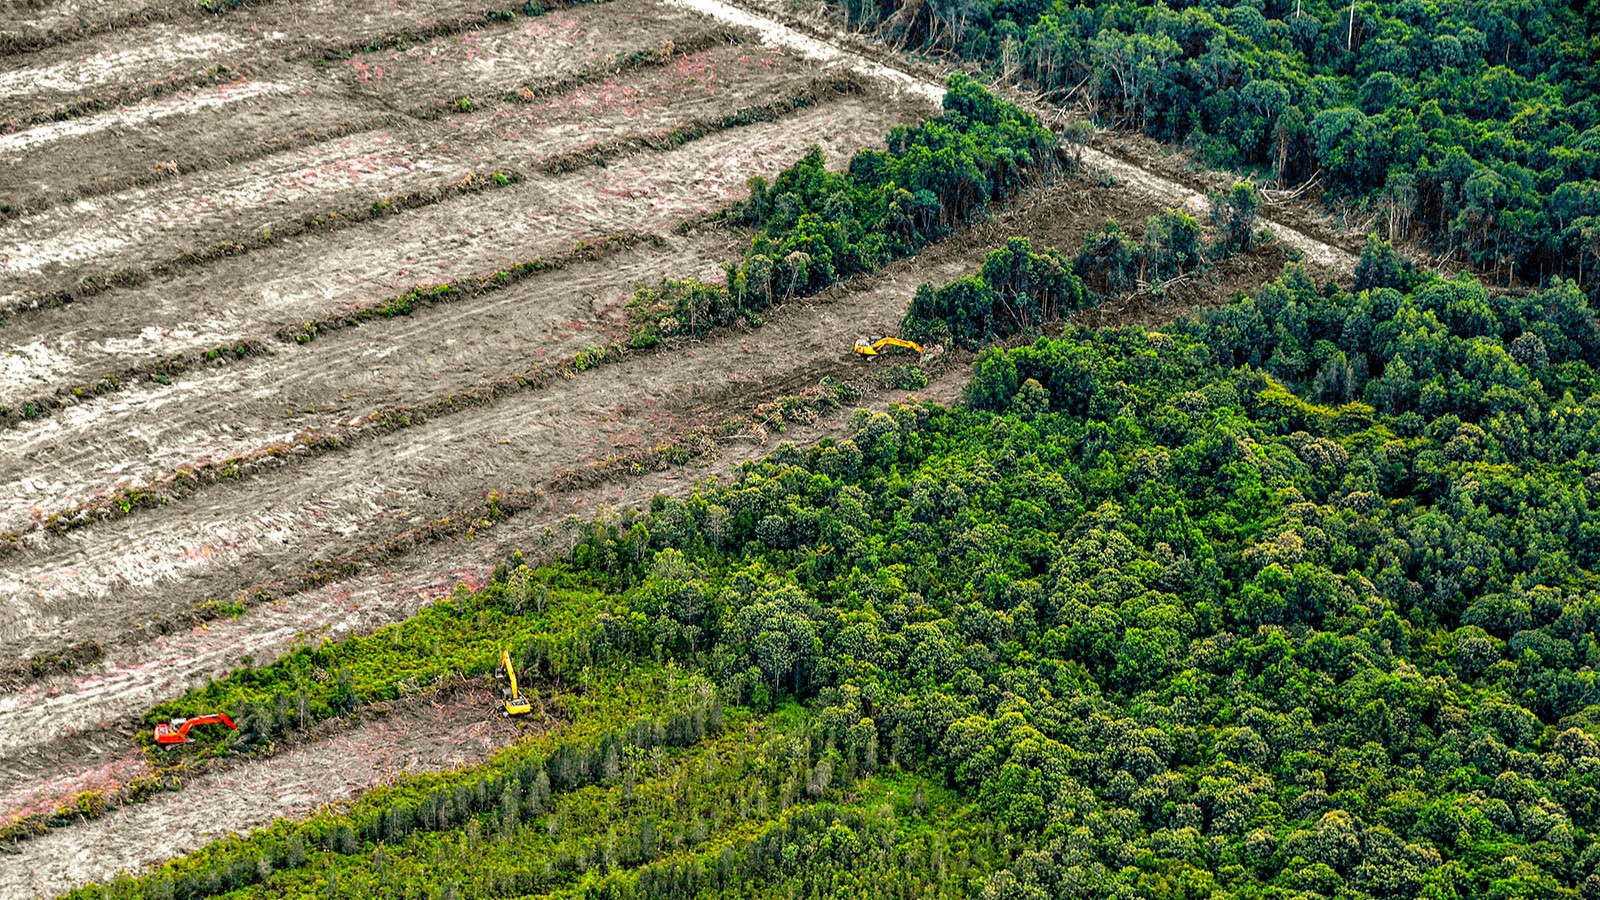
\includegraphics[height=4cm, keepaspectratio]{images/deforestation1.jpg} % 替换为你的第一张图片路径
            \caption{Deforestation for Farming}
            \label{fig:deforestation1}
        \end{minipage}
      \hspace{0.05\linewidth}
        \begin{minipage}[b]{0.45\linewidth}
            \centering
            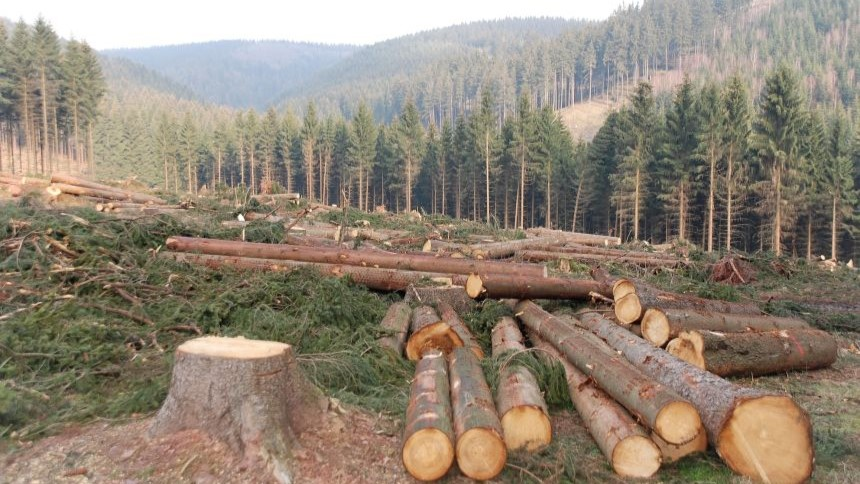
\includegraphics[height=4cm, keepaspectratio]{images/deforestation2.jpg} % 替换为你的第二张图片路径
            \caption{Deforested Forest}
            \label{fig:deforestation2}
        \end{minipage}
      \end{figure}
    Therefore, the converted forest area must undergo a long process of ecological reconstruction. 
    However, due to the influence of human activities during this process, 
    the post-clearing forest ecosystem can no longer return to its original state, 
    but instead continuously undergoes succession into a stable agricultural ecosystem. 
    To achieve both economic and ecological benefits and fulfill sustainable development goals, 
    it is necessary to examine the ecological succession from converted forest to agricultural ecosystems and explore how green agriculture can bring dual benefits in terms of economic and ecological indicators.
    \subsection{Problem Analysis}
      The basic requirements of the project are to establish a model that reflects the ecological succession process from a converted forest area to a mature agricultural ecosystem over time. 
      The model should incorporate both natural processes and human agricultural activities. 
      Specifically, the requirements are as follows:
      \begin{itemize}
        \item \textbf{Develop an ecological model} for the converted forest area, particularly:
          \begin{itemize}
            \item \textbf{Food web construction}: The model should include at least producers (e.g., plants) and consumers (e.g., herbivores and predators) and their interactions.
            \item \textbf{Consideration of agricultural cycles and seasonality}: The impact of seasonal and cyclical agricultural activities should be taken into account.
            \item \textbf{Impact of chemicals}: The model should account for the effects of chemicals such as herbicides and pesticides on plants, insects, bats, birds, and the stability of the ecosystem.
          \end{itemize}
        \item \textbf{Reemergence of species during ecosystem maturation}: As the ecosystem matures, the model should consider the reemergence of two species and their impact on the ecosystem.
        \item \textbf{Impact of removing chemicals}: After the ecosystem matures, humans will attempt to remove chemicals. The model should assess the stability of the ecosystem after herbicides are removed, with the effects reflected through producers and consumers.
        \item \textbf{Introduction of bats into the food web}: The model should examine how bats, as insectivores and pollinators, interact with plants, insects, and predators, and how their inclusion influences the stability of the ecosystem. Additionally, the model should identify another species that could benefit the ecosystem and compare the effects of different species.
        \item \textbf{Analysis of the impact of organic farming}: The model should assess the impact of adopting organic farming practices, considering various scenarios and components. The evaluation should include the effects on the overall ecosystem and individual elements, such as pest control, crop health, plant reproduction, biodiversity, long-term sustainability, and cost-effectiveness. The model should analyze the impact of organic practices on pest management, soil health, and biodiversity, while weighing the economic costs and benefits. A comprehensive ecological and economic trade-off analysis should be provided to assess the feasibility of organic farming.
      \end{itemize}
    \subsection{Our Work}
      To sum up the whole article, we have done the following work.
    \begin{itemize}
      \item Initially, we utilized difference equation to construct Model I: 
      LVLG Model, based on the Lotka-Volterra model and the Leslie-Gower model, 
      under the simplest food web conditions. This model considered producers, primary consumers, and secondary consumers.
      \item Subsequently, considering that ecosystem gradually developed, we built Model II: CAGED Model. 
      In this model, we incorporated agricultural cycle (three crops per year), 
      seasonal rotation (rainy and dry seasons), pollitation, Gussian noise, utilization of chemicals (herbicides and pesticides) and multiple digestion delays. 
      \item Next, we considered the reemergence of certain populations and their influence on the system. Specifically, we considered the reintroduction of snakes and frogs into the ecosystem, 
      which results in the formation of a more complex food web.
      \item After that, we introduced the SAGED Model to discuss the dynamics of ecosystems following farmers' adoption of green agricultural practices.
      \item We have created several agricultural production scenarios and applied the model developed above for practical analysis, 
      obtaining data that closely aligns with real-world conditions. 
      Our findings indicate that while chemical use can partially suppress weeds and pests, 
      the ecosystem's dependency on it is high and unstable. Reintroduction of species helps enrich the food web, 
      thereby stabilizing the ecosystem. 
      Ecological agriculture (e.g., introducing ducks and bats) is more conducive to ecosystem stability than chemical usage and offers long-term benefits. 
      \item We compared the effects of independently introducing ducks or bats as green agricultural methods on the ecosystem and analyzed integrated economic indicators. 
      Our findings show that green agriculture yields higher returns than chemical-based agriculture. 
      Ducks outperform bats in both promoting rice yield and overall economic profitability.
      \item We analyzed the stability of the model from both initial values and parameters. 
      We found that the model is insensitive to initial values but highly sensitive to parameters. 
      We attribute this to the fact that real-world ecosystems are capable of resisting external disturbances (initial values) and maintain stable intrinsic parameters, 
      which explains the model's high alignment with reality.
      \item Finally, based on our model and the data derived from it, we have written a letter of recommendations to farmers. 
      Specifically, we suggest agricultural measures that can maximize both economic and ecological benefits, 
      and outline policies that can effectively incentivize the sustainable development of agriculture.
    \end{itemize}
  \section{Assumptions and Notations}
    \subsection{Assumptions and Explanations}
      \begin{itemize}
        \item \textbf{Accurate Data Assumption}: The model assumes that the data used are accurate.\\
        \textbf{Explanation}: The data used in the model are sourced from official databases, and we believe the data to be accurate and reliable.
        \item \textbf{Geographic Applicability Assumption}: The model assumes that the applicable region is Southeast Asia,
         where two crops of rice are planted each year in the farmland.\\
        \textbf{Explanation}: The climate of Southeast Asia is rather simple, 
        with only two seasons-rainy and dry. Additionally, as is shown in \figurename~\ref{fig:Temperature},
        the temperature variation within a year is minimal, which has a trivial effect on the ecosystem.
        Consequently, temperature can be considered as a constant.
        Due to such weather pattern, it aligns with the planting patterns commonly observed in Southeast Asia to plant three crops of rice each year(showed in \figurename~\ref{fig:PlantMode}),
         and the simplicity of crop types makes the model easier to establish.
        \begin{figure}[H]
          \centering
          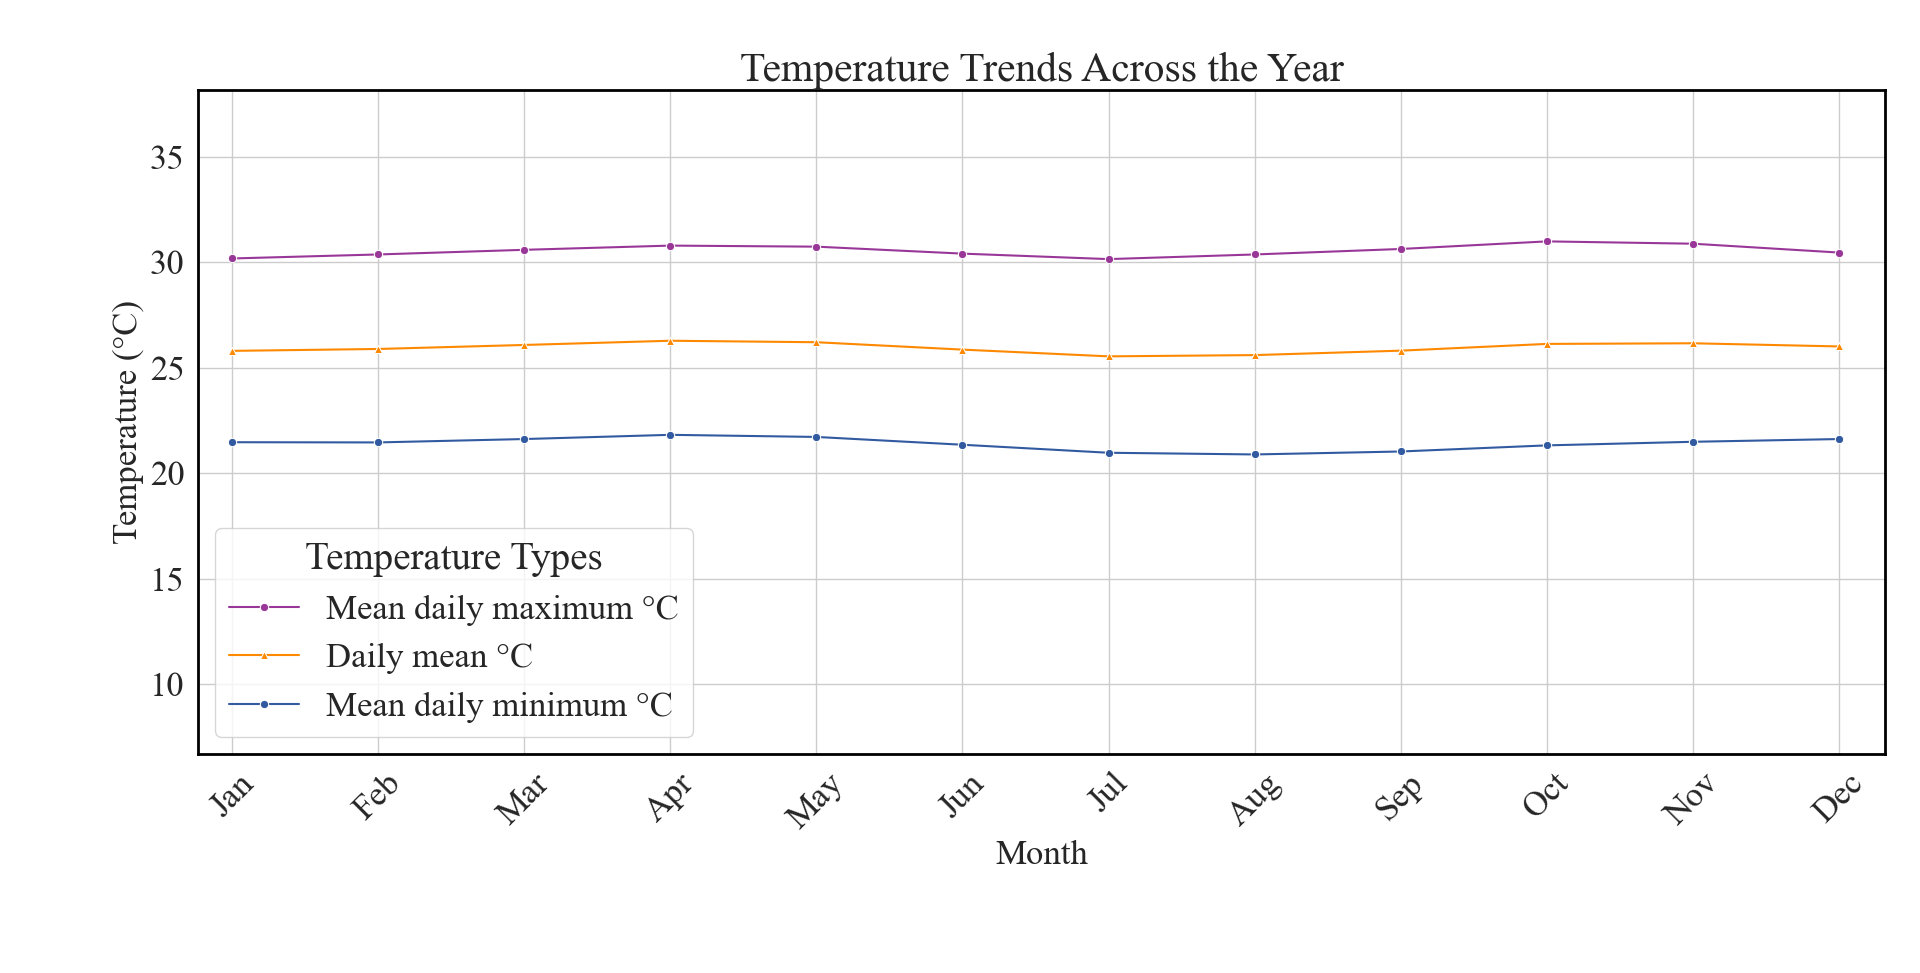
\includegraphics[width=0.75\linewidth]{images/AverTemper.png}
          \caption{Temperature Data in Southeast Asia\cite{IndoTemper}}
          \label{fig:Temperature}
        \end{figure}
        \begin{figure}[H]
          \centering
          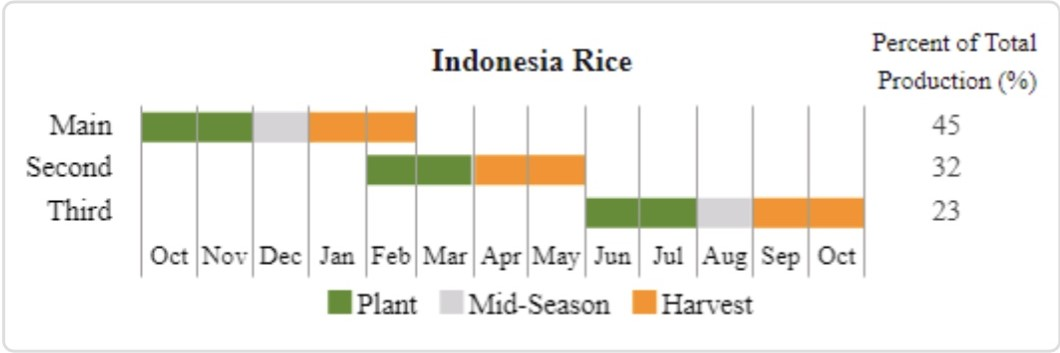
\includegraphics[width=0.75\linewidth]{images/PlantMode.jpg}
          \caption{Agricultural Cycle in Southeast Asia\cite{IndoRice}}
          \label{fig:PlantMode}
        \end{figure}
        \item \textbf{Stable Trait Assumption}: The model assumes that the traits of all organisms remain stable.\\
        \textbf{Explanation}:Since the time span considered in the model is much shorter than the time required for evolutionary changes or mutations to occur,
         the traits of organisms are assumed to remain stable. This assumption also helps simplify the model.
        \item \textbf{Stable Lighting Conditions Assumption}: The model assumes that the region under study experiences stable lighting conditions throughout the four seasons.\\
        \textbf{Explanation}: Since the model focuses on tropical regions, the variation in daylight duration across different months within a year is minimal,
         thus the lighting conditions are treated as constant in the model.
        \item \textbf{Stable Growth Environment Assumption}: The model assumes that no natural disasters,
         which could significantly impact the agricultural ecosystem, will occur during the time frame considered.\\
        \textbf{Explanation}: Natural disasters are considered low-probability events in agricultural activities.
         To ensure the generalizability of the model, natural disasters should not be considered.
      \end{itemize}
        \subsection{Notations}
      % table
      \begin{table}[H]
        \centering
        \caption{Notations}
        \begin{tabular}{cc}
          \toprule
          \rowcolor{customcolor!40} % 设置背景颜色
          Symbols & Description\\
          \midrule
          $wd, crp , stw$ & Subscription for weed, crop, straw respectively \\
          $ins, bd, bt, dk, snk, frg$ & Subscription for insect, bird, bat, duck, snake, frog respectively\\
          $HC, PC$ & Subscription for herbicide \\
          $C_i$ & Concentration of certain chemical \\
          $W_i$ & Density of biomass of certain species \\
          $r_i$ & Natural growth rate of certain population\\
          $\mathscr{K}_i$ & Biomass density carrying capacity of certain population\\
          $\alpha$ & The effect of chemical concentration on growth rate\\
          $\beta_{i \rightarrow j}$ & Interspecific competition factor\\
          $\gamma_{i \rightarrow j}$ & Percentage of i in j's total food consumption\\
          $A_{i\rightarrow j},B_{i\rightarrow j}$ & Effect of $i\rightarrow j$ pred-prey relationship on population $i$ \\
          $D_i,E_i$ & Effect of shortage of food on population $i$ \\
          \bottomrule
        \end{tabular}
        \label{tab:Notations}
      \end{table}
  \section{Models}
    \subsection{Notes for Model Development}
        Before building all the models, here are some notes for all the models.
        
        First, biomass is chosen over population density. This is because rice, 
        as the primary producer in the agricultural ecosystem, 
        has its population density artificially determined (i.e., it does not reproduce). 
        Only the changes in its total biomass can reflect the developmental trend of the rice population.
        
        Second, regarding interspecific competition, since the agricultural ecosystem is relatively simple compared to others, 
        for the sake of model simplification, only interspecific competition between rice and weeds is considered. 

        Next, for the purpose of further simplifying the model, some parameters are combined. 
        For example, the predation rate is incorporated into the predation coefficient of the prey species, denoted as \(A\).
        
        Finally, since consumers are in a natural reproductive state with a relatively fixed age structure, 
        the average individual biomass can be assumed to be constant. 
        Therefore, biomass is directly proportional to the number of individuals in the population.
        
        It should be noted that at the start time, all the variations and coefficients mentioned above are positive real numbers.
    \subsection{Model I: LVLG Model}
      LVLG Model represents the combination of Lotka-Volterra and Leslie-Gower Model. 
      Before establishing the model, We will first discuss the initial conditions of the model from the perspective of biological populations. 
      The vertical structure of tropical forests is typically divided into several layers, including the canopy layer, understory, shrub layer, and ground layer. 
      Each layer not only supports different plant species but also provides habitat and food sources for various animals. 
      
      Deforestation will severely disrupt the vertical structure of the tropical rainforest food web. 
      Therefore, our model assumes that at the initial time point following deforestation, 
      the vertical structure of the ecosystem above the ground retains only a portion of the ground layer. 
      All populations that previously depended on the canopy, understory, and shrub layers for habitat and food sources will have migrated out of the ecosystem.

      Based on this assumption, the agricultural ecosystem in its initial food web retains only the following populations: plants, insects, and birds. 
      First, to preserve interspecific competition and align with reality as closely as possible, we divide plants into two populations: rice and weeds. 
      Second, although insects may exhibit food preferences, for simplicity, we assume that there is only one insect species that feeds on both crops and weeds. 
      Finally, based on the feeding habits of birds in real life, we assume that birds feed on both insects and the two plant species. 
      \figurename~\ref{fig:LGVGField} presents a schematic diagram of the ecosystem, and \figurename~\ref{fig:SimpleFoodWeb} shows the initial food web of the ecosystem.
      \begin{figure}[H]
        \centering
          \begin{minipage}[b]{0.45\linewidth}
              \centering
              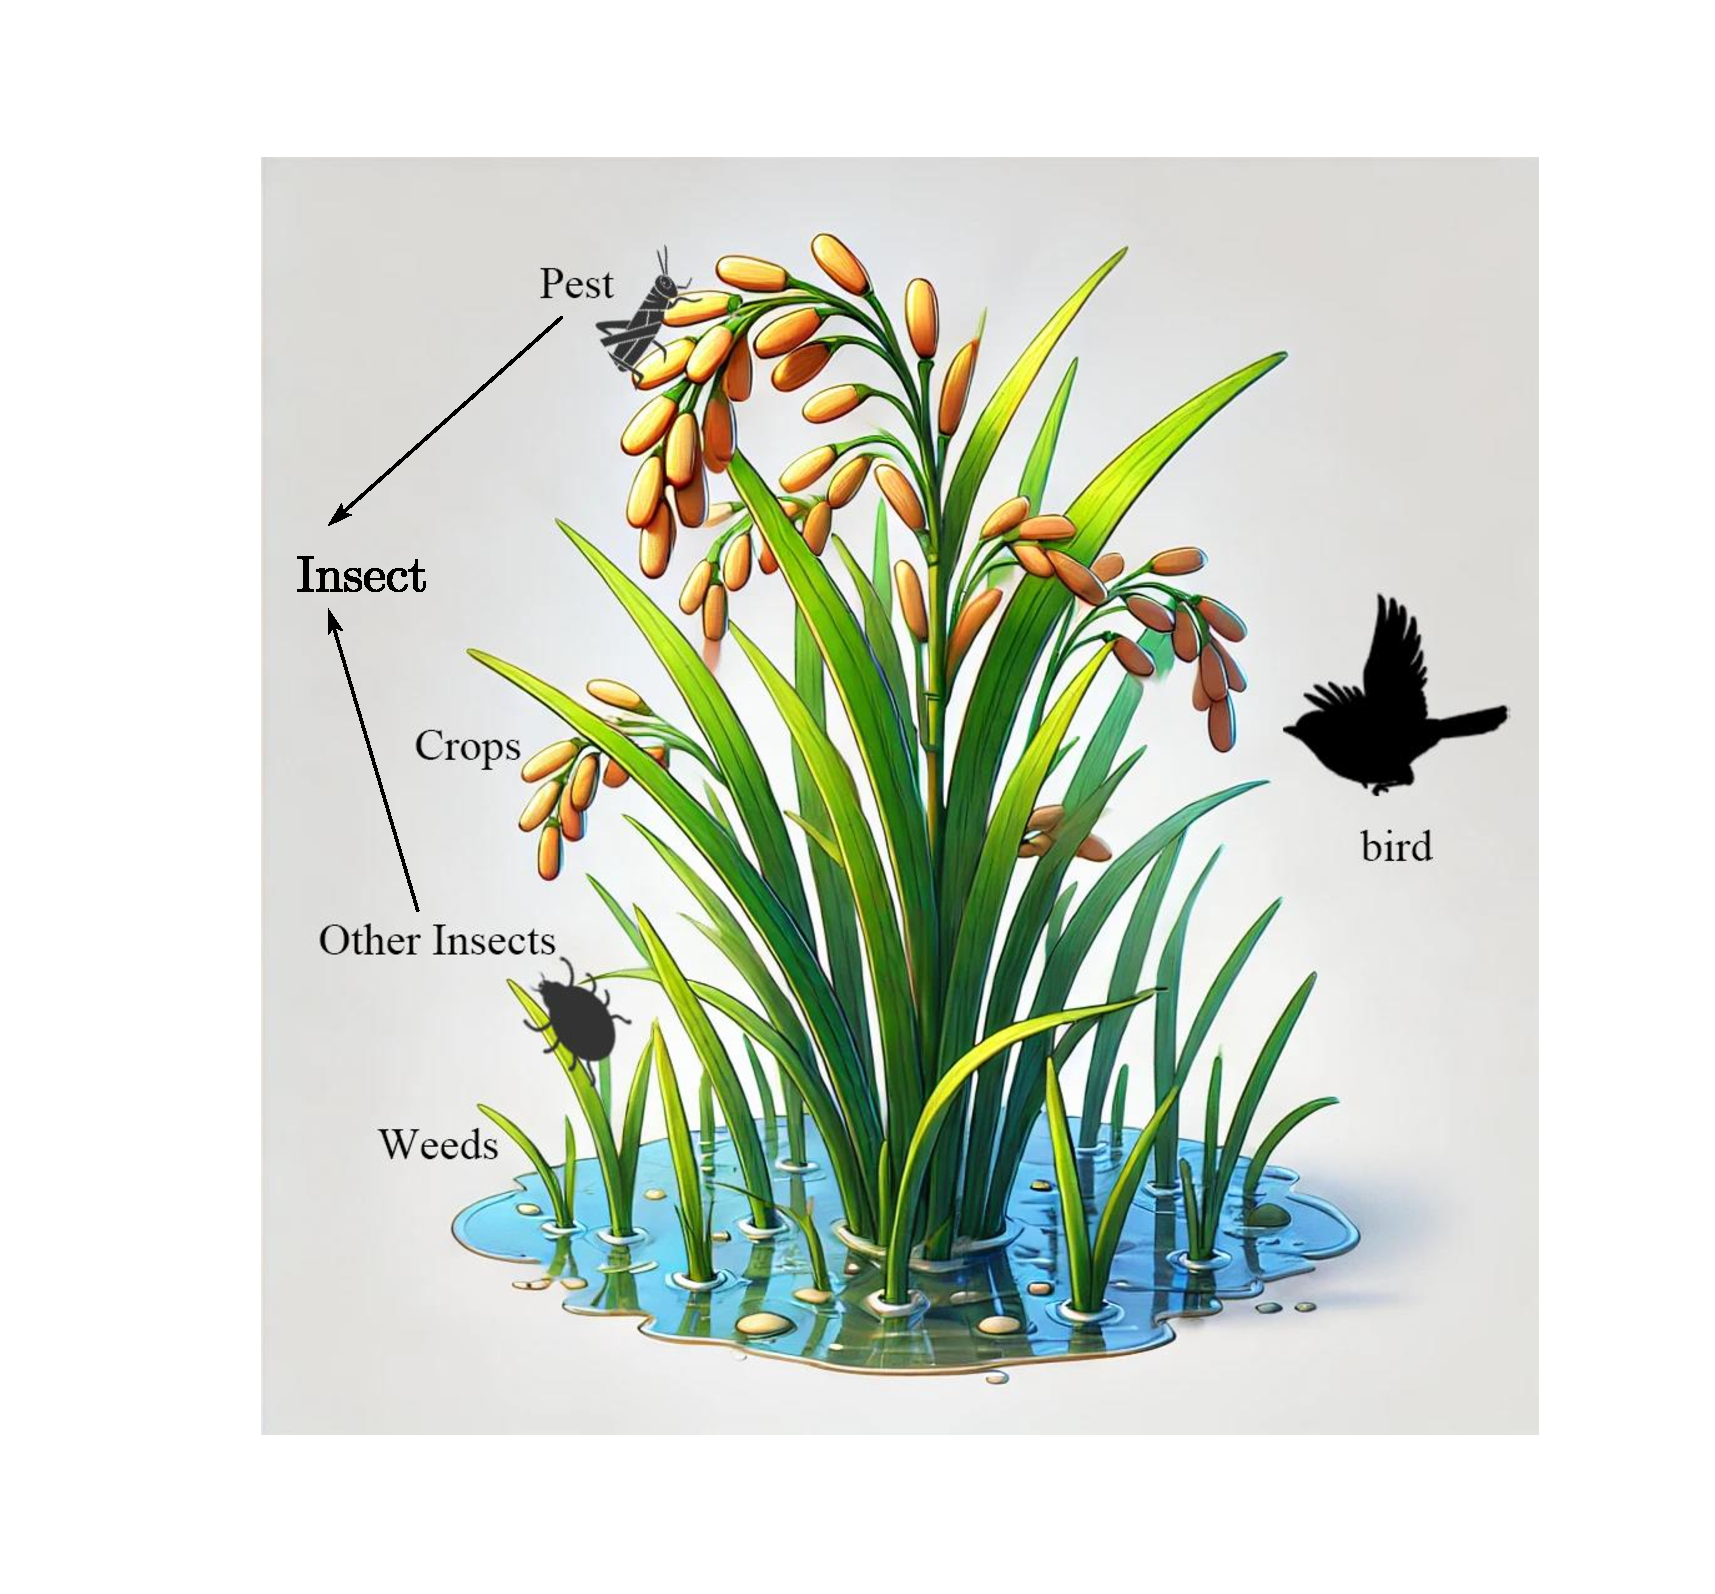
\includegraphics[height=5cm, keepaspectratio]{images/LGVGField.pdf} % 替换为你的第一张图片路径
              \caption{Schematic map for LGVG Model}
              \label{fig:LGVGField}
          \end{minipage}
        \hspace{0.05\linewidth}
          \begin{minipage}[b]{0.45\linewidth}
              \centering
              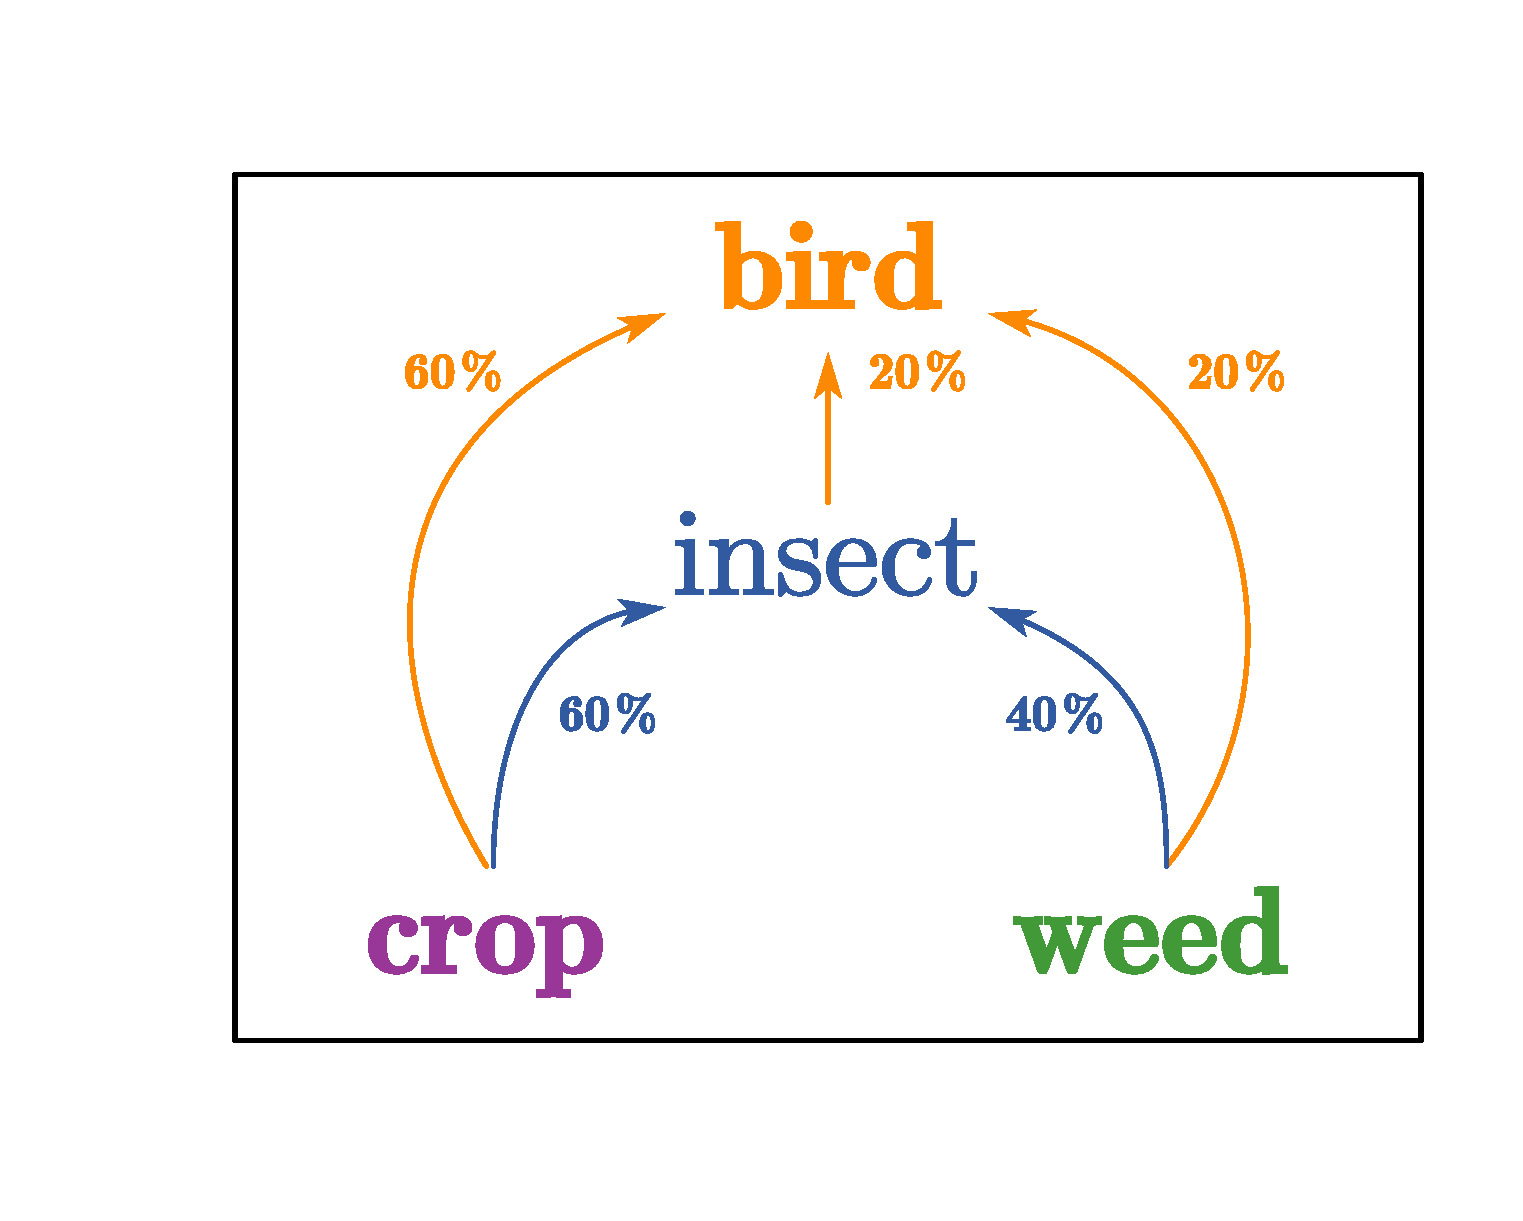
\includegraphics[height=5cm, keepaspectratio]{images/SimpleFoodWeb.pdf}
              \caption{Food web in LGVG Model}
              \label{fig:SimpleFoodWeb}
          \end{minipage}
        \end{figure}
      Set February-when rice has just been planted-as the start time.
      Around the start time, in the simplest case, when climate, soil, and other conditions are favorable, 
      only biological factors should be considered.
      If the population sizes of producers and primary consumers are used to describe the entire system, 
      the Lotka-Volterra Model\cite{wangersky1978lotka} and Leslie-Gower Model\cite{GUO20142850} can be applied as follows:

      \begin{equation}
        \begin{aligned}
          \frac{\mathrm{d}W_{crp}}{\mathrm{d}t}&=r_{crp}W_{crp}\left( 1-\frac{W_{crp}+\beta _{w\rightarrow c}W_{wd}}{\mathscr{K} _{crp}} \right) -\sum_{{j=pred}}{\frac{A_{crp\rightarrow j}W_{crp}W_{j}}{1+B_{crp\rightarrow j}W_{crp}}}\\
          \frac{\mathrm{d}W_{wd}}{\mathrm{d}t}&=r_{wd}W_{wd}\left( 1-\frac{W_{wd}+\beta _{c\rightarrow w}W_{crp}}{\mathscr{K} _{wd}} \right) -\sum_{{j=pred}}{\frac{A_{wd\rightarrow j}W_{wd}W_{j}}{1+B_{wd\rightarrow j}W_{wd}}}\\
          \frac{\mathrm{d}W_{ins}}{\mathrm{d}t}&=r_{ins}W_{ins}\left[ 1-\frac{D_{ins}W_{ins}}{1+E_{ins}\left( 0.6W_{crp}+0.4W_{wd} \right)} \right] -\frac{A_{ins\rightarrow bd}W_{ins}W_{bd}}{1+B_{ins\rightarrow bd}W_{ins}}\\
          \frac{\mathrm{d}W_{bd}}{\mathrm{d}t} &= r_{bd}W_{bd} \left[ 1 - \frac{D_{bd}W_{bd}}{1 + E_{bd}(0.2W_{ins} + 0.2W_{wd} + 0.6W_{crp})} \right]\\
        \end{aligned} 
      \end{equation}

      In general, these four equations introduce the natural growth term $r_i W_i$ for population growth. 
      The first two equations incorporate the interspecific competition term $\beta_{i \rightarrow j} W_i$, 
      the larger this term, the more intense the interspecific competition, and the slower the biomass growth rate of population $i$. 
      
      For population $i$, the first three equations consider the effect of predation($i\rightarrow j$, which means $j$ hunts $i$) through the term 
      
      \begin{equation}
      \sum_{j=pred}{\frac{A_{i\rightarrow j}W_{i}W_{j}}{1+B_{i\rightarrow j}W_{i}}}
      \end{equation}
      
      In the term above, we can see that when the biomass of predators(here, namely, insects and birds) increases, 
      the rate of increasing of certain prey will recude due to the hunting effects.

      The last two equations(e.g. the third one) include the term 

        \begin{equation}
          \frac{D_{i} W_{i}}{1 + E_{i} \sum_{j=food}{\gamma_{j\rightarrow i} W_{j}}},
        \end{equation}

          which represents biomass reduction due to food scarcity. 
      In the denominator, one factor is weighted according to the predation ratio: the less food available, 
      the more predators there are, resulting in a slower growth rate of the predator population.
    \subsection{Model II: CAGED Model}
      CAGED Model represents Conprehensive Agro-Ecosystem Dynamics Model, and it is the core model of the hole article.
      Model I is quite simple and aims to construct a basic short-term model. 
      Considering the impact of long-term environmental factors, 
      in order to better simulate the long-term evolutionary behavior of the ecosystem model, 
      we will progressively introduce the effects of simplified agricultural cycles, 
      seasonality, soil fertility, pollination, random factors and multiple digestion delays on the system dynamics model. 
      Furthermore, we will consider the impact of chemical use, 
      specifically the application of herbicides and pesticides, on the system, 
      building upon this natural agricultural ecosystem model.
      \subsubsection{Agricultural Cycle}
        According to rice production in Indonesia(\figurename~\ref{fig:PlantModePlus}), 
        rice production in Southeast Asia follows a three-crop-per-year pattern. 
        We assume that February, June, and October are the overlapping periods of two agricultural cycles 
        (from the last post-harvest period to the new planting period).
        \begin{figure}[H]
          \centering
          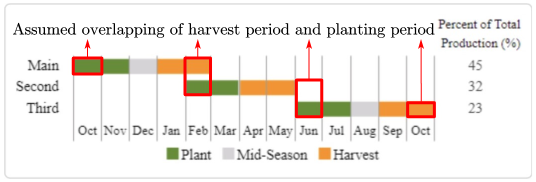
\includegraphics[width=0.7\linewidth]{images/PlantModePlus.png}
          \caption{Overlapping Periods of Two Agricultural Cycles}
          \label{fig:PlantModePlus}
        \end{figure}
        During the overlapping period, the rice population re-enters the food web in the form of seeds after harvesting, 
        starting a new agricultural cycle. The mature rice straw, as an agricultural byproduct, 
        remains in the ecosystem after harvesting, and after being treated by methods such as burning or returning to the field, 
        the rice biomass is decomposed and ingested by decomposers and insects, ultimately decreasing to zero.

        Based on literature review\cite{OLIVER20191139,summers2003biomass}, 
        the biomass fate of mature rice during each overlapping period can be uniformly described by \figurename~\ref{fig:rice_to}. 
        \begin{figure}[H]
          \centering
          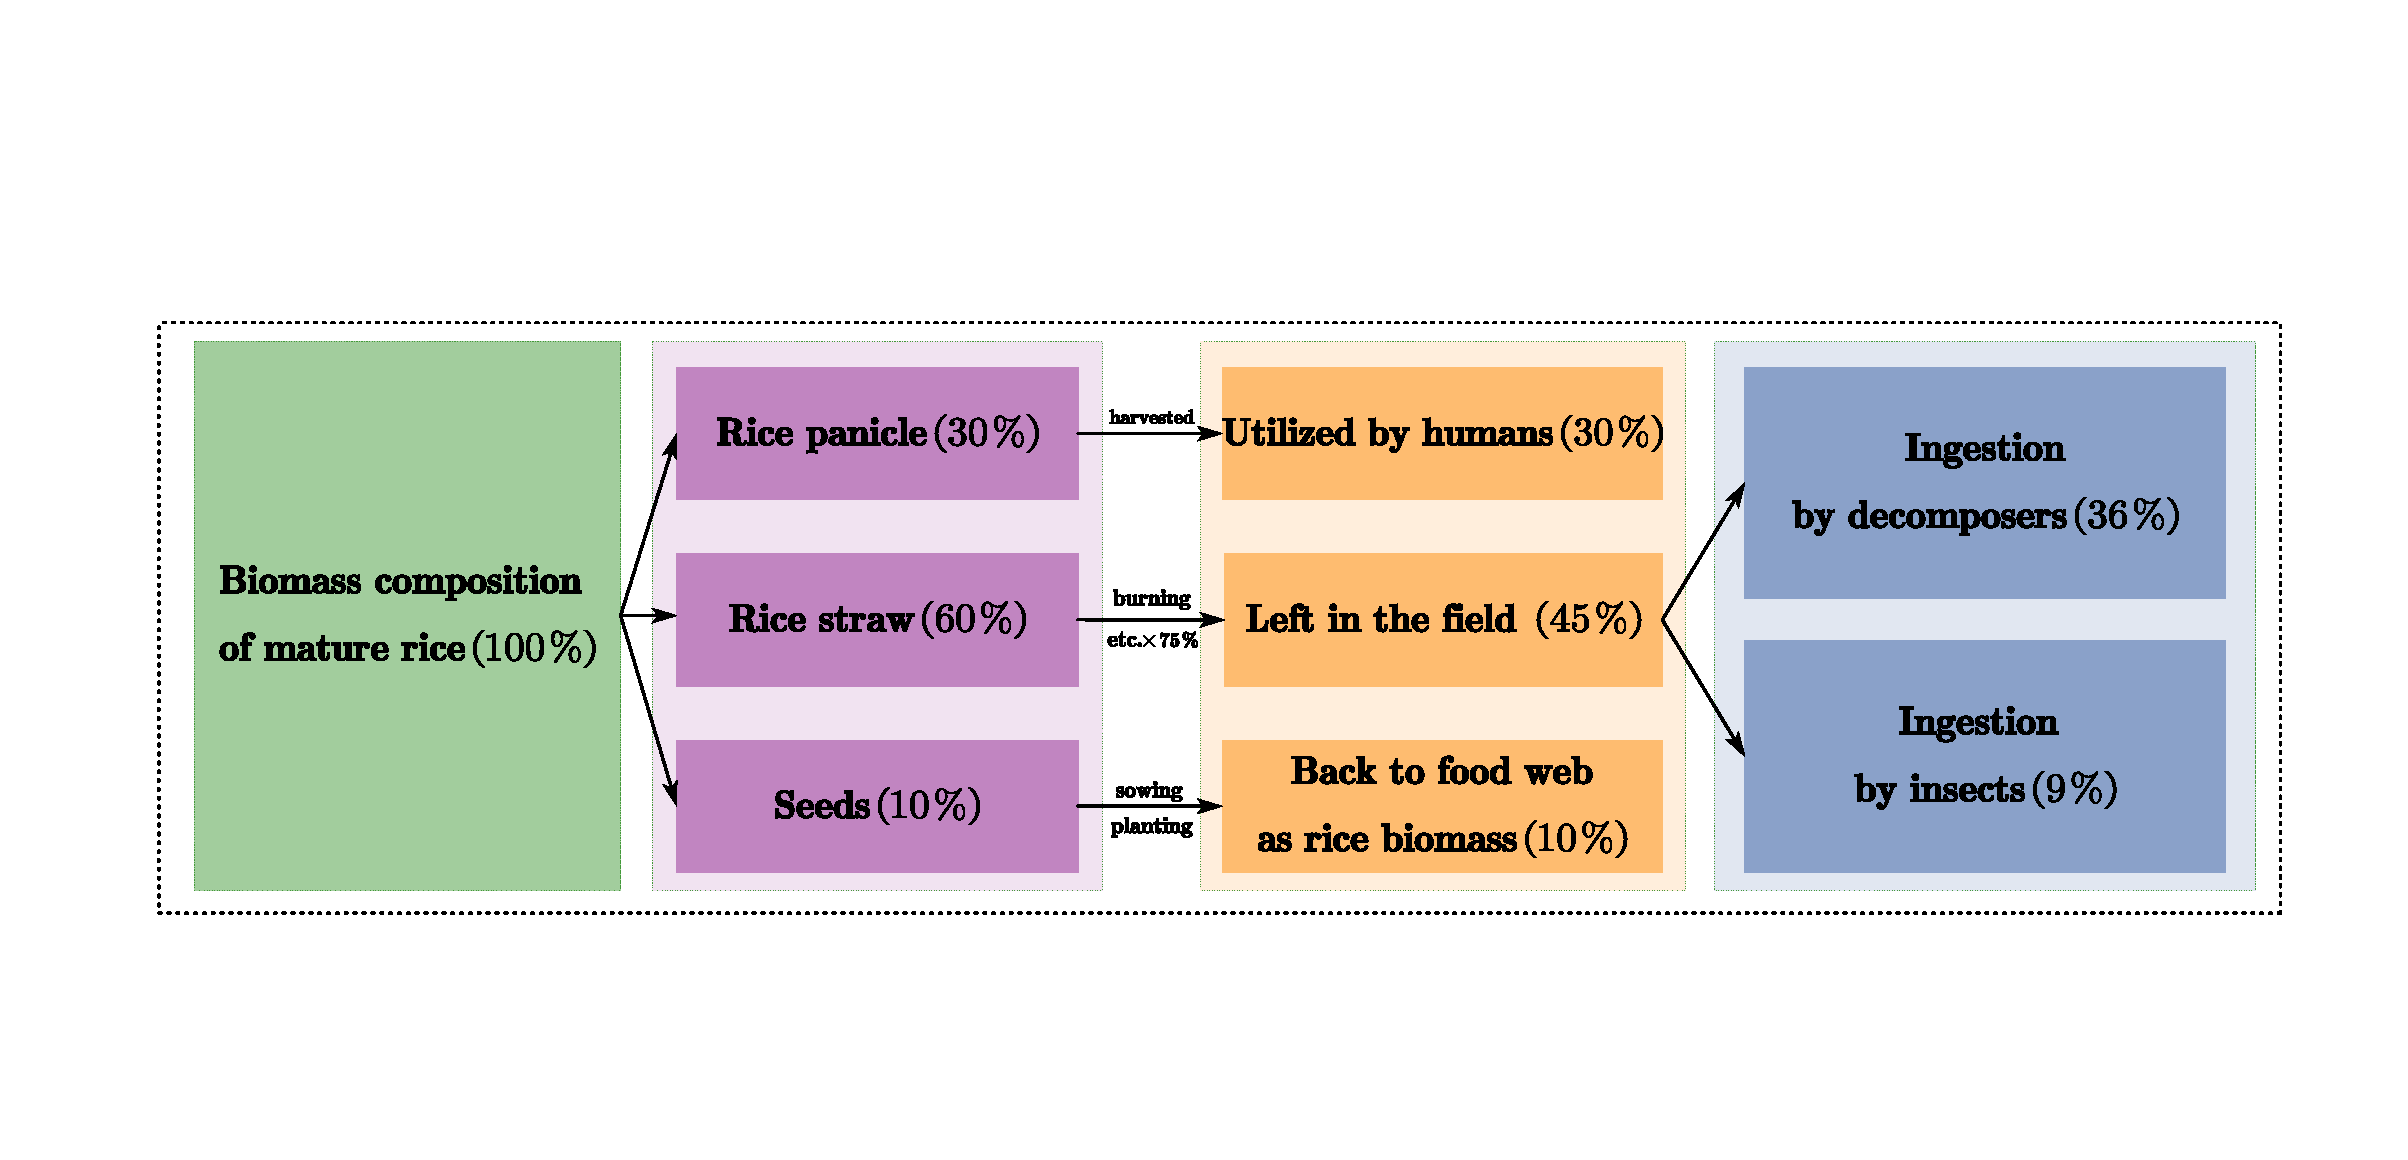
\includegraphics[width=\linewidth]{images/rice_to.pdf}
          \caption{Biomass Fate of Mature Rice during Each Overlapping Period}
          \label{fig:rice_to}
        \end{figure}
        Since decomposers' biomass is not considered in our food web model, 
        we only analyze the impact of decomposed rice straw residue(the 36\% part) on the producers—namely rice and weeds—in the new cycle. 
        For further details, refer to the soil fertility section later in the paper.
      
        For simplification of the model, 
        the biomass change of the rice population during each overlapping period is represented 
        by a biomass step function at specific time points in the mathematical model (i.e., the system of difference equations). 
        Since $t=0$ corresponds to the start of the first planting season, with one year assumed to have 52 weeks, 
        and each week being a time step, based on the rice production pattern \figurename~\ref{fig:PlantModePlus}, 
        we define the step moments at week 0, week 17, and week 34 of each year. The biomass of rice at these times follows:

        \begin{equation}
        W_{crp}|_{t=n}=0.1W_{crp}|_{t=n-1}, \quad n = 52k, 52k+17, 52k+34, \quad (year\, k \geqslant 0, \, week\, n \geqslant 1)
        \end{equation}

        When considering the impact of rice straw on insect biomass, 
        we treat rice straw as the 'prey' of insects and use the modified Lotka-Volterra (LG) predator-prey model to characterize this effect. 
        At each step moment, rice straw enters the food web model with an initial biomass of $0.09W_{crp}$, and $r_{stw} = 0$. 
        Thus, the rice straw-insect model is established as:

        \begin{equation}
          \frac{\mathrm{d}W_{stw}}{\mathrm{d}t} = \frac{A_{stw\rightarrow ins} W_{stw} W_{ins}}{1 + B_{stw\rightarrow ins} W_{stw}} \quad (t \neq n)
        \end{equation}

        \begin{equation}
          W_{stw}|_{t=n} = W_{stw}|_{t=n-1} + 0.09 W_{crp}|_{t=n-1},
        \end{equation}
        
        \begin{equation}
          n = 52k, 52k+17, 52k+34, \quad (k \geqslant 0, \, n \geqslant 1, k,n\ are\ positive\ integers)
        \end{equation}
        The difference equation for insect biomass is modified as follows:
        \begin{equation}
          \frac{\mathrm{d}W_{ins}}{\mathrm{d}t} = r_{ins} W_{ins} \left[ 1 - \frac{D_{ins} W_{ins}}{1 + E_{ins} \left( 0.6 W_{crp} + 0.4 W_{wd} + W_{stw} \right)} \right] - \frac{A_{ins\rightarrow bd} W_{ins} W_{bd}}{1 + B_{ins\rightarrow bd} W_{ins}}
        \end{equation}

      \subsubsection{Seasonality}
        The seasonal influences primarily include factors such as light, 
        climate (temperature, precipitation), and biological habits, 
        all of which have significant direct effects on both $r$ and $\mathscr{K}$ within populations. 
        Considering that many of these factors are difficult to quantify precisely, 
        we set sinusoidal perturbations in the periodic parameter $p(T)$ as follows\cite{GAKKHAR20061239}:

        \begin{equation}
          p(t) = \bar{p} \left[ 1 + \epsilon \sin (\Omega t + \phi) \right]
        \end{equation}

        Specifically, in the LV-LG model mentioned above, 
        for population $i$, the values of $r_i$ and $K_i$ are defined as follows:

        \begin{align}
          r_i &= \bar{r}_i \left[ 1 + \epsilon_i \sin \left( \Omega_i t + \phi_i \right) \right] \\
          \mathscr{K}_i &= \bar{\mathscr{K}}_i \left[ 1 + \epsilon_i \sin \left( \Omega_i t + \phi_i' \right) \right], \quad \left( i = \text{crp or wd} \right) \\
          D_i &= \frac{\bar{D}_i'}{1 + \epsilon_i \sin \left( \Omega_i t + \phi_i' \right)}, \quad \left( i \neq \text{crp or wd} \right)
        \end{align}

        Where $\bar{r}_i$ and $\bar{\mathscr{K}}_i$ are the corresponding periodic means, 
        which can be treated as constants; $\Omega_i$ is the seasonal fluctuation angular frequency, 
        and $T = \frac{2\pi}{\Omega}$ is the seasonal fluctuation period; 
        $\epsilon_i$ is the seasonal impact parameter. Since $r_i, \mathscr{K}_i \geqslant 0$, 
        it follows that $-1 \leqslant \epsilon_i \leqslant 1$; $\phi_i$ and $\phi_i'$ are the phases, 
        with $0 \leqslant \phi_i < 2\pi$, which characterize the asynchronous fluctuations of biomass in different species.

        It can be mathematically proven that, after incorporating these variations, 
        the LV-LG model system theoretically possesses non-trivial stable points when the parameters are within a certain range. 
        When the system is near these points, the ecosystem can recover from small perturbations, 
        reaching a dynamic ecological equilibrium.
      \subsubsection{Soil Fertility}
        Now, we introduce the effect of soil fertility on plant growth.
        $i$ in the following statements represents rice or weed, $j$ the other.
        For the sake of simplicity in the model, 
        the influence of soil fertility on plant growth is divided into two main factors: 
        the effect of carbon dioxide (CO$_2$) concentration and the concentration of inorganic salts absorbed by the plants.

        Regarding the CO$_2$ concentration term, 
        since the agricultural ecosystem is an open system and, 
        in our context, can be considered to be surrounded by a vast and complex forest ecosystem, 
        the impact of respiration from the components of the agricultural ecosystem on the atmospheric CO$_2$ concentration can be neglected. 
        Thus, the CO$_2$ concentration is approximated as a constant, \( C_{CO_2} \). 
        Based on this, we introduce the soil fertility factor \( \mu_{Fr_i} = f(C_{Is_i}) \). 
        Soil fertility has a complex and profound effect on parameters such as the growth rate of population biomass, 
        competition coefficients, and the maximum carrying capacity of the environment. 
        An important consideration here is the effect of \( \mu \) on the environmental maximum biomass carrying capacity, 
        as shown below:

        \[
        \frac{\mathrm{d}W_{i}}{\mathrm{d}t} = r_{i} W_{i} \left( 1 - \frac{W_{i} + \beta_{j \rightarrow i} W_{j}}{\mathscr{K}_{i} \cdot \mu_{Fr_i}} \right) - \sum_{j=pred}{\frac{A_{i\rightarrow j} W_{i} W_{j}}{1 + B_{i\rightarrow j} W_{i}}}
        \]

        For the inorganic salt concentration term, 
        it is closely related to fertilizer concentration (which is influenced by straw and chemical fertilizers), 
        decomposer activity, and the growth stage of the plant. Taking rice as an example: when rice reaches the seedling stage, 
        its internal inorganic salt concentration is low, and the growth acceleration of the concentration is positive; 
        during the tillering to jointing stage, the demand for inorganic salts increases rapidly, and the concentration reaches a turning point; 
        during the booting to flowering stage, the rate of increase in inorganic salt concentration slows down until it reaches its maximum; 
        during the milk-ripe and yellow-ripe stages, the absorption of inorganic salts decreases gradually, and the concentration drops.\cite{garcia2003logistic}
        
        We use a Gaussian-like probability density function to fit the trend of the inorganic salt concentration in the plant over each agricultural cycle, given by:
        
        \[
        C_{Is_i}(t) = \alpha_{Is_i} e^{-\frac{(t - T_{mc})^2}{\sigma_{Is_i}}}
        \]

        where \( T \) represents the time at which the concentration of inorganic salts in rice or weeds is at its maximum during a cycle; the remaining two parameters correspond to the model constants for rice or weeds, 
        and are determined by fertilizer concentration (from both chemical fertilizers and straw), decomposer activity, and the plant's growth stage.

        Again, for the sake of model simplification, we assume \( \mu_{Fr_i} = \xi_{i} C_{Is_i} \).
      \subsubsection{Random Factors}
        Considering the influence of random factors in nature, we introduce Gaussian white noise \(\sigma_i\) for each population.
        
        The probability density function of the Gaussian white noise \(\sigma_i(t) = x\) is given by:

        \begin{equation}
        f(x) = \frac{1}{\sqrt{2\pi\sigma^2}} e^{-\frac{x^2}{2\sigma^2}}
        \end{equation}

        which means that \(\sigma_i\) follows a normal distribution with a mean of 0.
        
        Our generation method is as follows:
        \begin{itemize}
            \item Generate two distinct random functions \(U_1(t)\) and \(U_2(t)\) within the interval \([0, 1]\);
            \item Take \(\eta(t) = -\sqrt{-2 \ln U_1(t)} \cdot \cos(2\pi U_2(t))\), which gives \(\eta(t)\) as the Gaussian white noise function.
        \end{itemize}
        The noise corresponding to different species in the equations is shown in \figurename~\ref{fig:GussianNoise}.
        \begin{figure}[H]
          \centering
          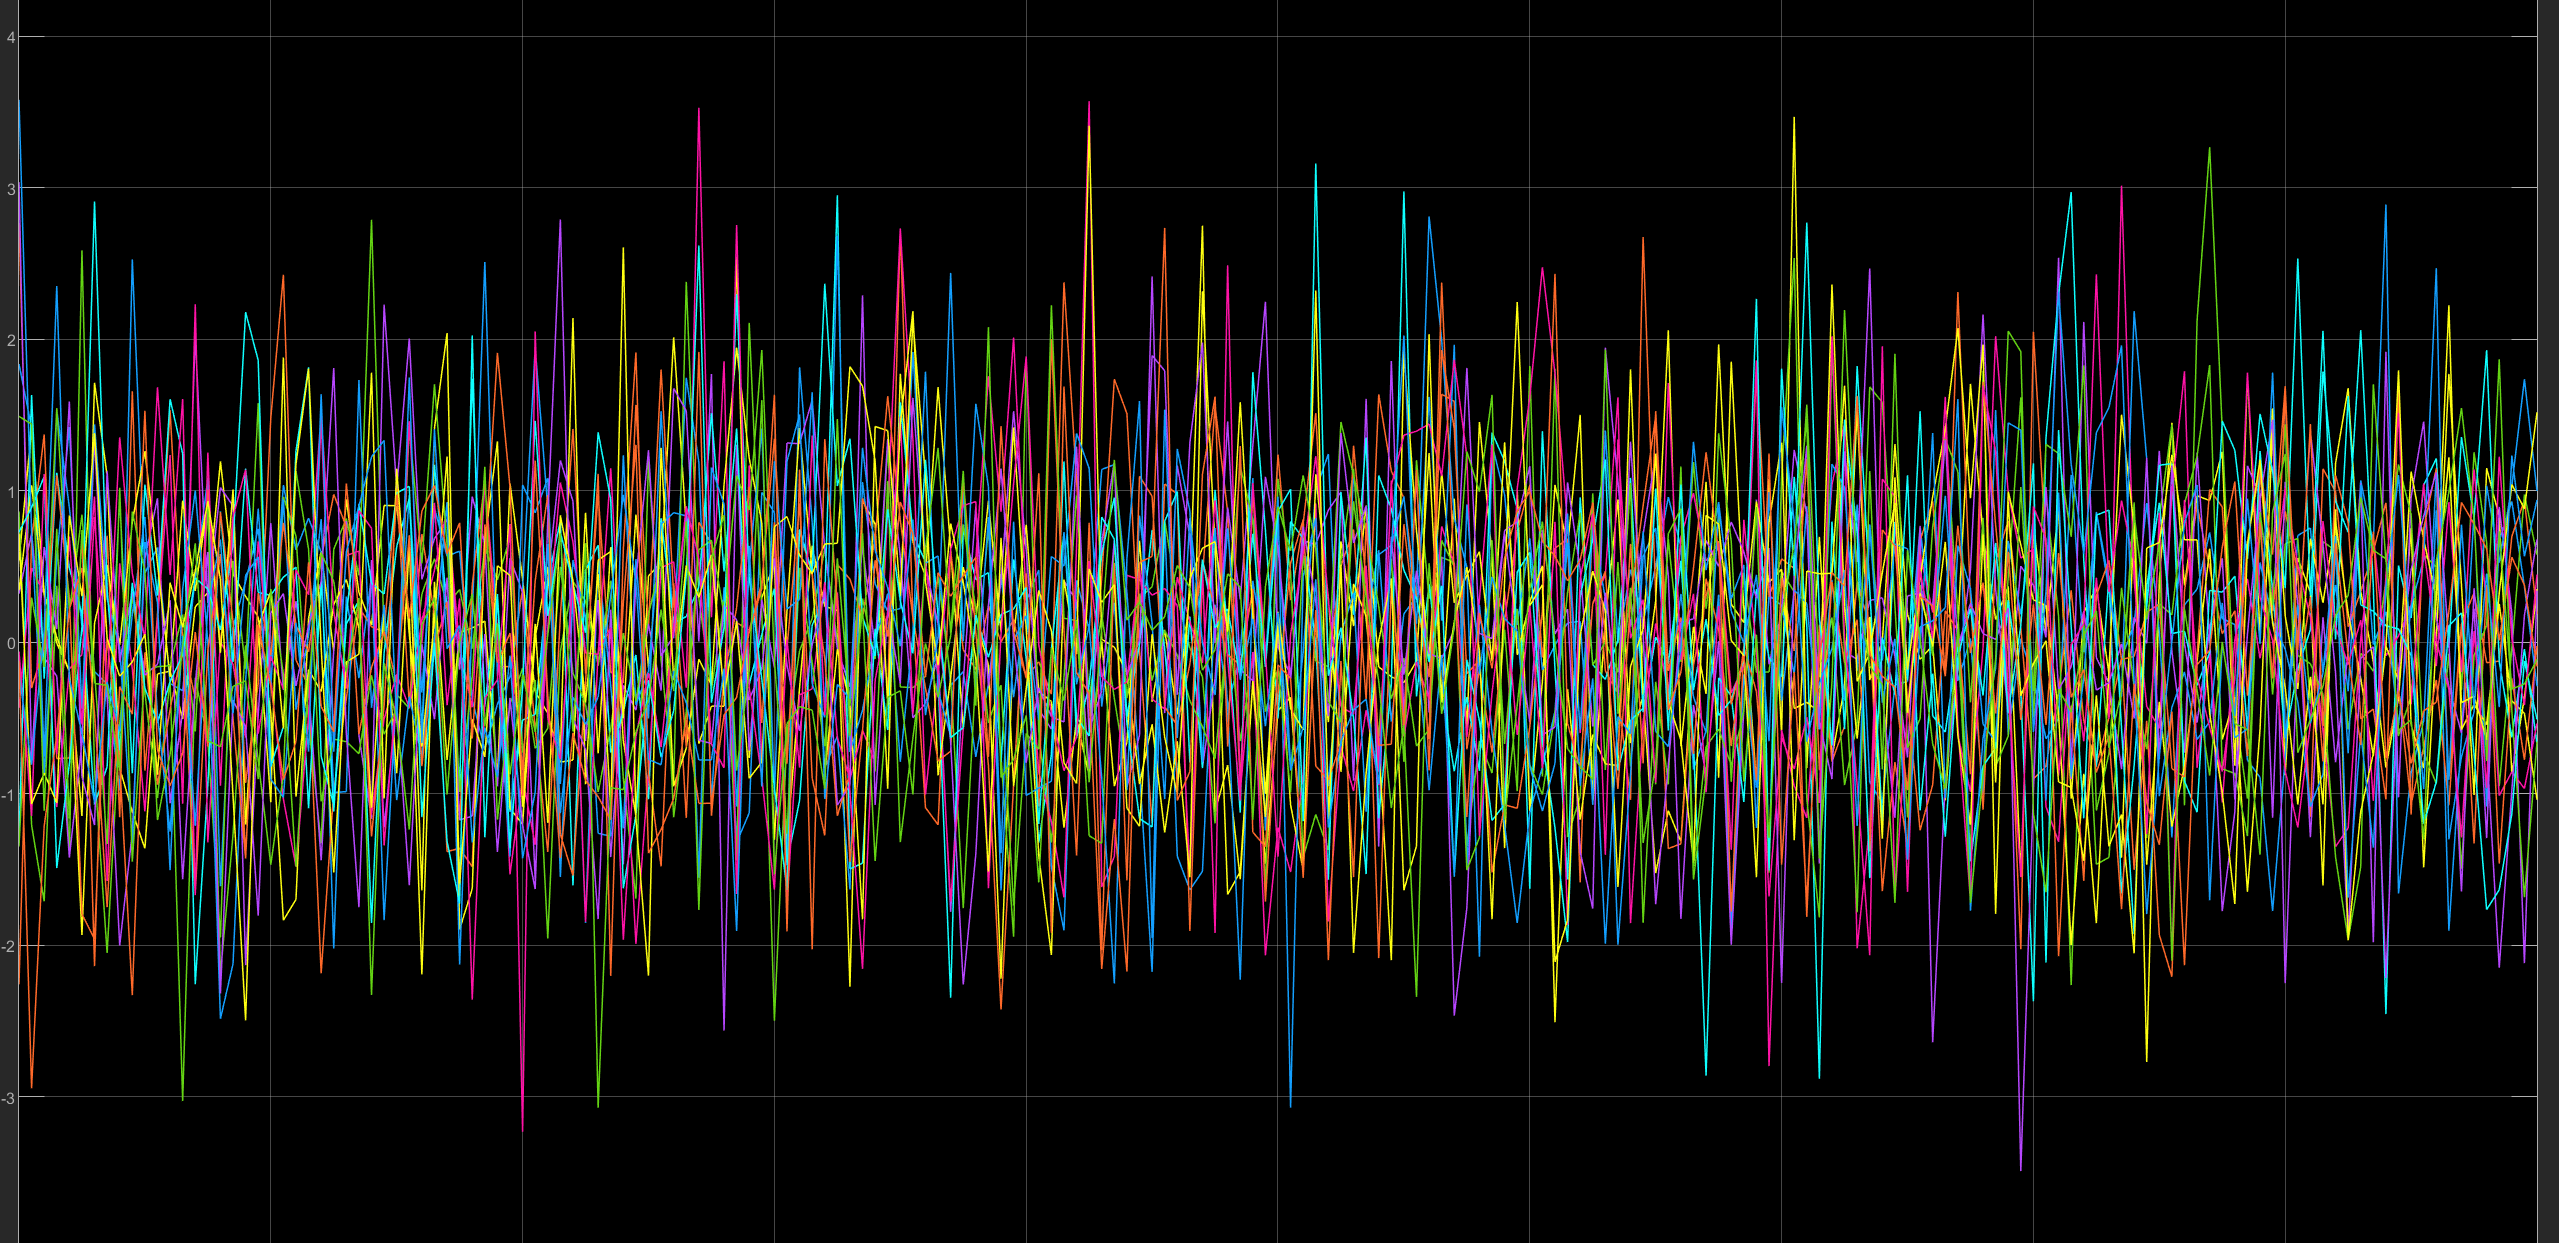
\includegraphics[width=0.5\linewidth]{images/GussianNoise.png}
          \caption{Gussian Noises of Each Population}
          \label{fig:GussianNoise}
        \end{figure}
      \subsubsection{Chemical Use}
        For herbicides, considering that the application times of herbicides during rice cultivation are primarily before sowing, 
        at the seedling stage, and at the tillering stage, we assume that herbicides are applied three times during an agricultural cycle, 
        with the application occurring at weeks 0, 3, and 8. The herbicide concentration is proportional to the current weed biomass. 
        Since the application frequency is relatively low, we can ignore the specific negative effects of herbicides on rice 
        (any minor negative effects can be covered by the random process described in random factors).

        We consider weeds as the "prey" of the herbicides. 
        Similarly to the straw-insect model mentioned earlier, we can use the modified Lotka-Volterra predator-prey model, where \( r_n \equiv 0 \).
      
        For the degradation of the herbicide, we can use an exponential decay model. Thus, we establish the weed-herbicide model as follows:
      
        \begin{equation}
        C_{hc}|_{t=m} = C_{hc}|_{t=m-1} + \alpha_{uh} W_{wd}|_{t=m},
        \end{equation}
        \begin{equation}
        \frac{dW_{wd}}{dt} = r_{wd}W_{wd} \left( 1 - \frac{W_{wd} + \beta_{c \rightarrow w} W_{crp}}{\mathscr{K}_{wd}} \right) - \sum_{j=pred}{\frac{A_{wd\rightarrow j} W_{wd} W_{j}}{1 + B_{wd\rightarrow j} W_{wd}}} - \frac{A_{hc} W_{wd} C_{hc}}{1 + B_{hc} W_{wd}},
        \end{equation}
        \begin{equation}
        \frac{dC_{hc}}{dt} = - \alpha_{dh} C_{hc}.
        \end{equation}
        
        For insecticides, we can establish an insect-insecticide model that follows a similar mechanism to the weed-herbicide model. 
        We set the insecticide application times during an agricultural cycle to be at week 4, week 8, and week 12. Unlike the weed-herbicide model, 
        since there are pests that primarily feed on rice and other insects that primarily feed on weeds, 
        and the insecticide has a much more significant effect on eliminating pests than on eliminating other insects, 
        the food composition of insects as a whole changes after insecticide application. Specifically, 
        the proportion of rice in their diet decreases significantly, while the proportion of weeds increases significantly. 
        Based on this, we introduce the parameter \( \lambda_{pc} \), which is dominated by the insecticide concentration, 
        to describe the impact of the insecticide on the insect food composition as follows:
        
        \begin{equation}
          C_{pc}|_{t=m} = C_{pc}|_{t=m-1} + \alpha_{up} W_{ins}|_{t=m}, 
        \end{equation}

        \begin{equation}
          \begin{split}
            \frac{dW_{ins}}{dt} = r_{ins} W_{ins} &\left( 1 - \frac{D_{ins} W_{ins}}{1 + E_{ins} \left[ (0.6 - \lambda_{pc}) W_{crp} + (0.4 + \lambda_{prc}) W_{wd} \right]} \right) \\
            &-\frac{A_{ins\rightarrow bd} W_{ins} W_{bd}}{1 + B_{ins\rightarrow bd} W_{ins}} - \frac{A_{pc} W_{ins} C_{pc}}{1 + B_{pc} W_{ins}},
          \end{split}
      \end{equation}

        \begin{equation}
        \frac{dC_{hc}}{dt} = - \alpha_{dp} C_{hc}.
        \end{equation}
      
      \subsubsection{Multiple Digestion Delay}
        Due to the time required for energy flow, 
        the impacts of different predation relationships in the food web on system dynamics are actually asynchronous \cite{GUO20142850}. 
        Considering this asynchrony, 
        we introduce multiple digestion delays corresponding to the digestion periods of the consumer-eat-producer and predator-eat-consumer interactions, 
        referred to as the producer digestion delay (PDD) and consumer digestion delay (CDD), respectively.

        Mathematically, the PDD and CDD influence the food scarcity term \(L_i\) in the differential equation corresponding to the consumer population \(i\):
        
        \begin{equation}
        L_i = -r_i \frac{D_i W_i^2}{1 + E_i \cdot \Sigma_{\text{food}} \gamma_i W_{i_j}}
        \end{equation}

        where \(\Sigma_{\text{food}} \gamma_i W_{i_j}\) is the weighted sum of the biomass of the populations preyed upon by \(i\), weighted by the predation ratio. 
        After considering the delay, this term is modified as follows and incorporated into the original differential equation:
        
        \begin{equation}
        L_i' = -\frac{r_i}{t - \tau_i} \cdot \frac{D_i W_i^2}{1 + E_i \cdot \Sigma_{\text{food}} \gamma_i W_{i_j}}
        \end{equation}

        where \(\tau_i\) is the digestion delay factor of population \(i\), and \(D_i, E_i\) are the corresponding environmental parameters for population \(i\).
    \subsection{CAGED Model Considering Restatement}
      As the ecosystem gradually matures, previously existing populations will re-enter the system. We assume that when the biomass of the prey species reaches a certain threshold (a tunable parameter), the species will migrate into the ecosystem, forming a more complex food web. In our model, we only consider the migration of frogs and snakes. After their migration, the previously constructed equations are applicable to describe their biomass dynamics (assuming they are not affected by chemicals).
    \subsection{Model III: SAGED Model}
      SAGED Model represents sustainable Agro-Ecosystem Dynamics Model.
      When the food web becomes sufficiently complex, humans can begin making agricultural decisions. The agricultural decision considered in our model involves removing herbicides and insecticides, while introducing bats and ducks.

      Bats play a role in promoting pollination; thus, the pollination factor becomes:
      
      \[
      f_{pd} = \begin{cases}
      1, & \text{non-pollinating period}, \\
      f_0 + c_1 W_{ins} + c_2 W_{bt}, & \text{pollinating period}.
      \end{cases}
      \]
      
      Besides this, the modified model only requires the removal of chemicals from the CAGED model, and the introduction of two new populations to form the ultimate food web.

  \section{Appication of the Models}
    The process of model establishment has been thoroughly presented in the previous subsection. 
    In this subsection, we will discuss the application of the models.
    In the models below, the unit of biomass(considering the entire farm) is kg and the unit of time is week.
        
    It should be noted that the graph contains some data points that are less than zero. These values are a result of the interpolation algorithm and do not represent actual negative biomass. 
        The interpolation process sometimes generates small negative values due to the smoothing of data points, 
        especially at the boundaries of the data set or during transitions between different states of the system. 
        These negative values should be interpreted as artifacts of the numerical method and not as realistic biological quantities.
    \subsection{Selection of Parameters}
      After reviewing the literature and aligning the parameters with their real-world significance, 
      we have determined a series of parameters. Due to the large number of parameters, 
      we present the table for the main ones:
      \begin{table}[H]
        \centering
        \caption{Parameters}
        \begin{tabular}{cc}
          \toprule
          \rowcolor{customcolor!40} % 设置背景颜色
          Symbols & Description\\
          \midrule
          $123$ & 123\\
          \bottomrule
        \end{tabular}
        \label{tab:Parameters}
      \end{table}
      All of the following models will apply these parameters. 
      
      \subsection{Scenarios Statement}
        Scenarios are stated in Table \ref{tab:Scenarios}, where S represents Scenario, Y for Yes and N for No.

        \begin{table}[H]
          \centering
          \caption{Scenarios}
          \begin{tabular}{lcccccccc}
            \toprule
            \rowcolor{customcolor!40} % 设置背景颜色
            conditions & S1 & S2 & S3 & S4 & S5 & S5A & S5B & S6 \\
            \midrule
            Agro-Activities & Y & Y & Y & Y & Y & Y & Y & Y \\
            Seasonality & Y & Y & Y & Y & Y & Y & Y & Y \\
            Chemicals & N & Y & Y & N & N & N & N & N \\
            Reemergence & N & N & Y & Y & Y & Y & Y & Y \\
            Bat & N & N & N & N & Y & Y & N & N \\
            Duck & N & N & N & N & Y & N & Y & N \\
            other methods & N & N & N & N & N & N & N & Y \\

            \bottomrule
          \end{tabular}
          \label{tab:Scenarios}
        \end{table}
      \subsection{Comparison between S1 and S2: Effects of Chemicals}

      The biomass densities of producers and consumers in S1 and S2 are shown in Figure \ref{fig:S1S2}, respectively.

      \begin{figure}
      \centering
      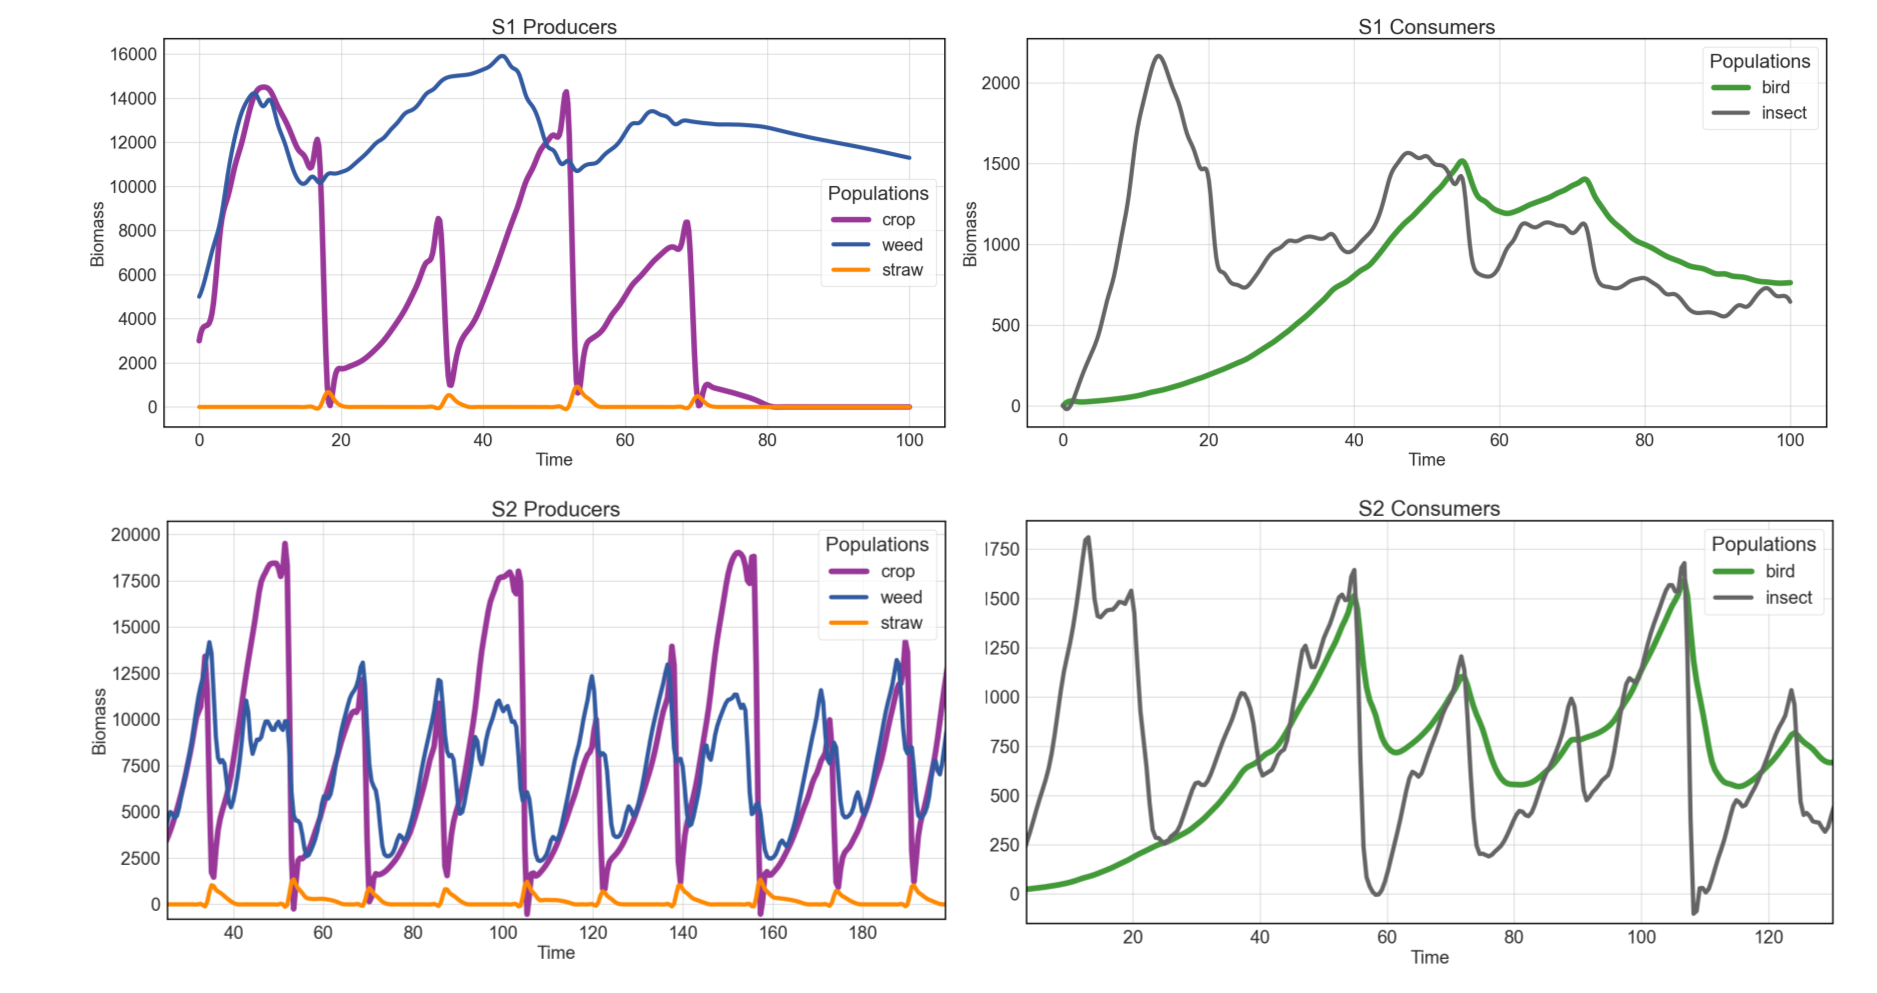
\includegraphics[width=\linewidth]{images/S1S2.png}
      \caption{Comparison between S1 and S2}
      \label{fig:S1S2}
      \end{figure}
      
      Analysis reveals that under S1, the ecosystem develops normally; 
      however, rice cannot survive in the long term, and thus, the system cannot evolve into an agricultural ecosystem. 
      This suggests that rice has weak competitive abilities against weeds and poor resistance to pests, 
      making it unable to persist in the ecosystem without human intervention.
      
      In the early stages of the agricultural ecosystem, before species re-migrate, 
      the model corresponds to S2. At this point, the ecosystem develops normally, 
      rice can survive in the long term, and the system gradually evolves into a mature agricultural ecosystem. 
      This indicates that the traditional chemical-agriculture model is capable of maintaining an agricultural ecosystem. 
      
      Furthermore, it has been clearly shown that S2 shows more complex and regular behavior compared to S1, 
      which indicates that S2 is more suitable for agriculture due to its regularity.
      
      \subsection{Comparison between S2 and S3: The Role of Species Migration}
        After the ecosystem has evolved for a certain period, external species re-migrate, the food web could be seen in Figure \ref{fig:food_web_chem}. 
        We compare S2 (early development) and S3 (mature development) to examine the ecosystem's stability.
        The dynamic behaviors of the S2 and S3 systems are shown in Figure \ref{fig:S2S3}.
        \begin{figure}
          \centering
          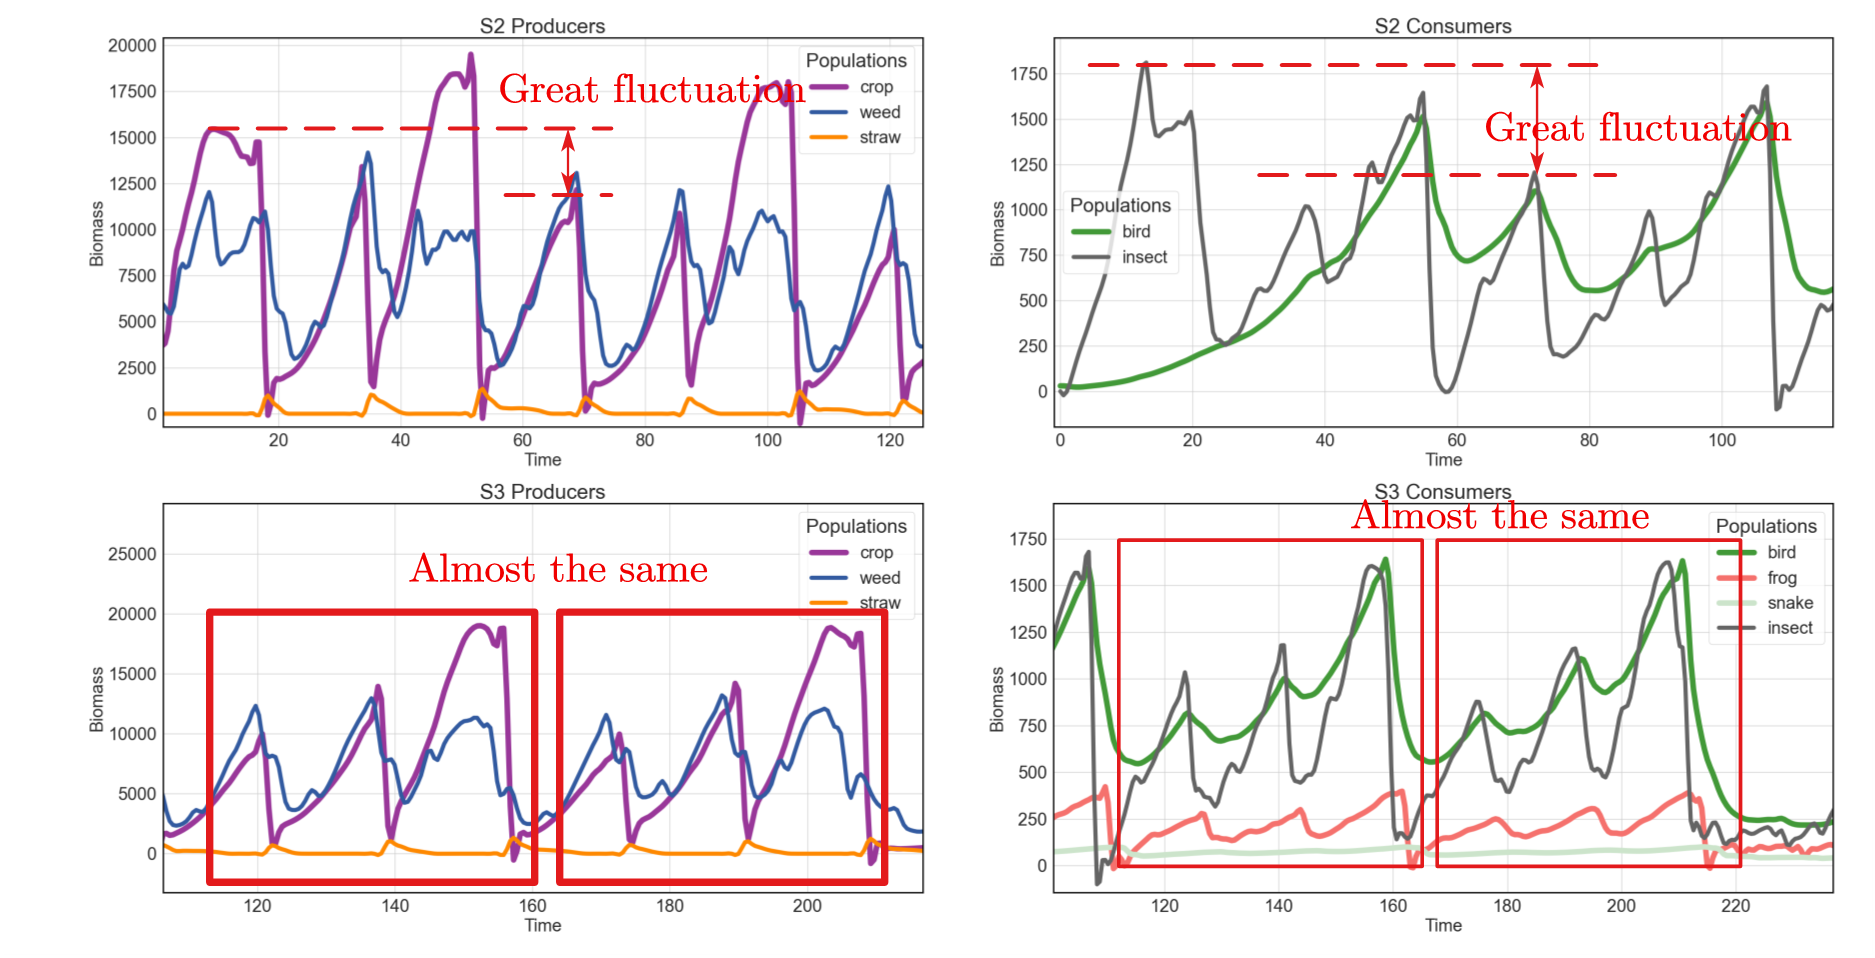
\includegraphics[width=\linewidth]{images/S2S3.png}
          \caption{Comparison between S2 and S3}
          \label{fig:S2S3}
        \end{figure}

        By comparing the two situations, we can observe that before considering the migration of other species, 
        the ecosystem in S2 exhibits some periodic fluctuations. However, the amplitude of these fluctuations is large, 
        and the system cannot remain at a stable level. After considering the migration of other species, 
        the ecosystem in S3 shows almost identical system states in each cycle, presenting a very stable pattern. 
        The above comparison indicates that when the migration of other species is taken into account, 
        the evolutionary pattern of the ecosystem becomes more stable, forming highly regular periodic changes. 
        This can be explained by the niche theory: as the food web becomes more complex, 
        even if a particular population is disturbed, 
        other species overlapping with its niche can temporarily take over its ecological role, 
        thus maintaining the normal functioning of the ecosystem.

      \subsection{Comparison between S3 and S4: The Dependency of the Chemical-Agriculture Model on Chemicals}
      After species migration, we consider removing chemicals and compare the ecosystem's situation in the two periods. 
      The result is shown in Figure \ref{fig:S4}.
      \begin{figure}
        \centering
        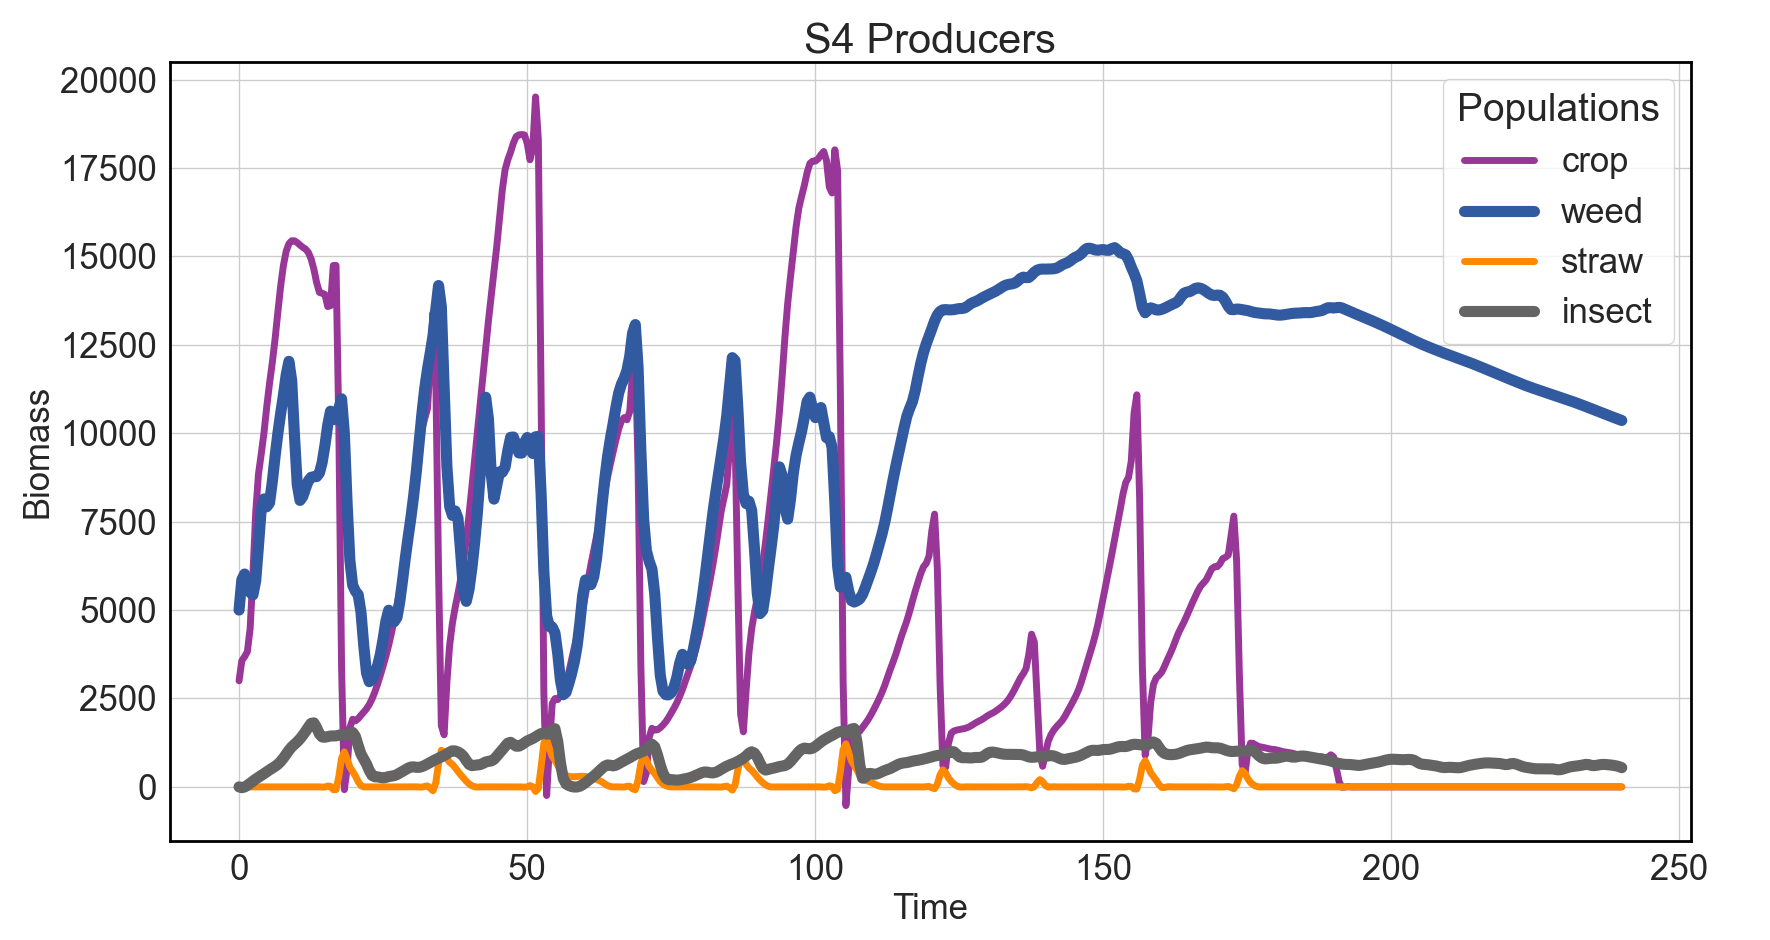
\includegraphics[width=0.7\linewidth]{images/P4_producers.png}
        \caption{Dynamics after Removing Chemicals}
        \label{fig:S4}
      \end{figure}
      
      By comparing the two situations, we find that in the traditional chemical-agriculture model, 
      the agricultural ecosystem is highly dependent on chemicals. Once chemicals are removed, 
      rice begins to lose out in competition with weeds, while pest interference increases. 
      The agricultural ecosystem's output gradually decreases, 
      and the ecosystem becomes increasingly unsuitable for agricultural activities.
      
      \subsection{Comparison between S3 and S5: The Superiority of the Green Agriculture Model}
        When the agricultural ecosystem has fully matured, 
        we can consider adopting green agricultural measures. In this case, 
        we examine the effect of introducing biological agents as replacements for chemicals, 
        specifically ducks and bats. The characteristics of ducks and bats are as follows:
        \begin{itemize}
            \item Ducks' physiological structure prevents them from consuming rice, but they can feed on weeds and pests.
            \item Ducks are introduced two weeks after each planting season, and they are harvested synchronously with rice at the end of the season.
            \item Bats are introduced once, serving as both pollinators and insect predators.
        \end{itemize}
        When introduced simultaneously, the final food web is shown in Figure \ref{fig:food_web_green}.
        
        \begin{figure}[H]
          \begin{minipage}[b]{0.45\linewidth}
            \centering
            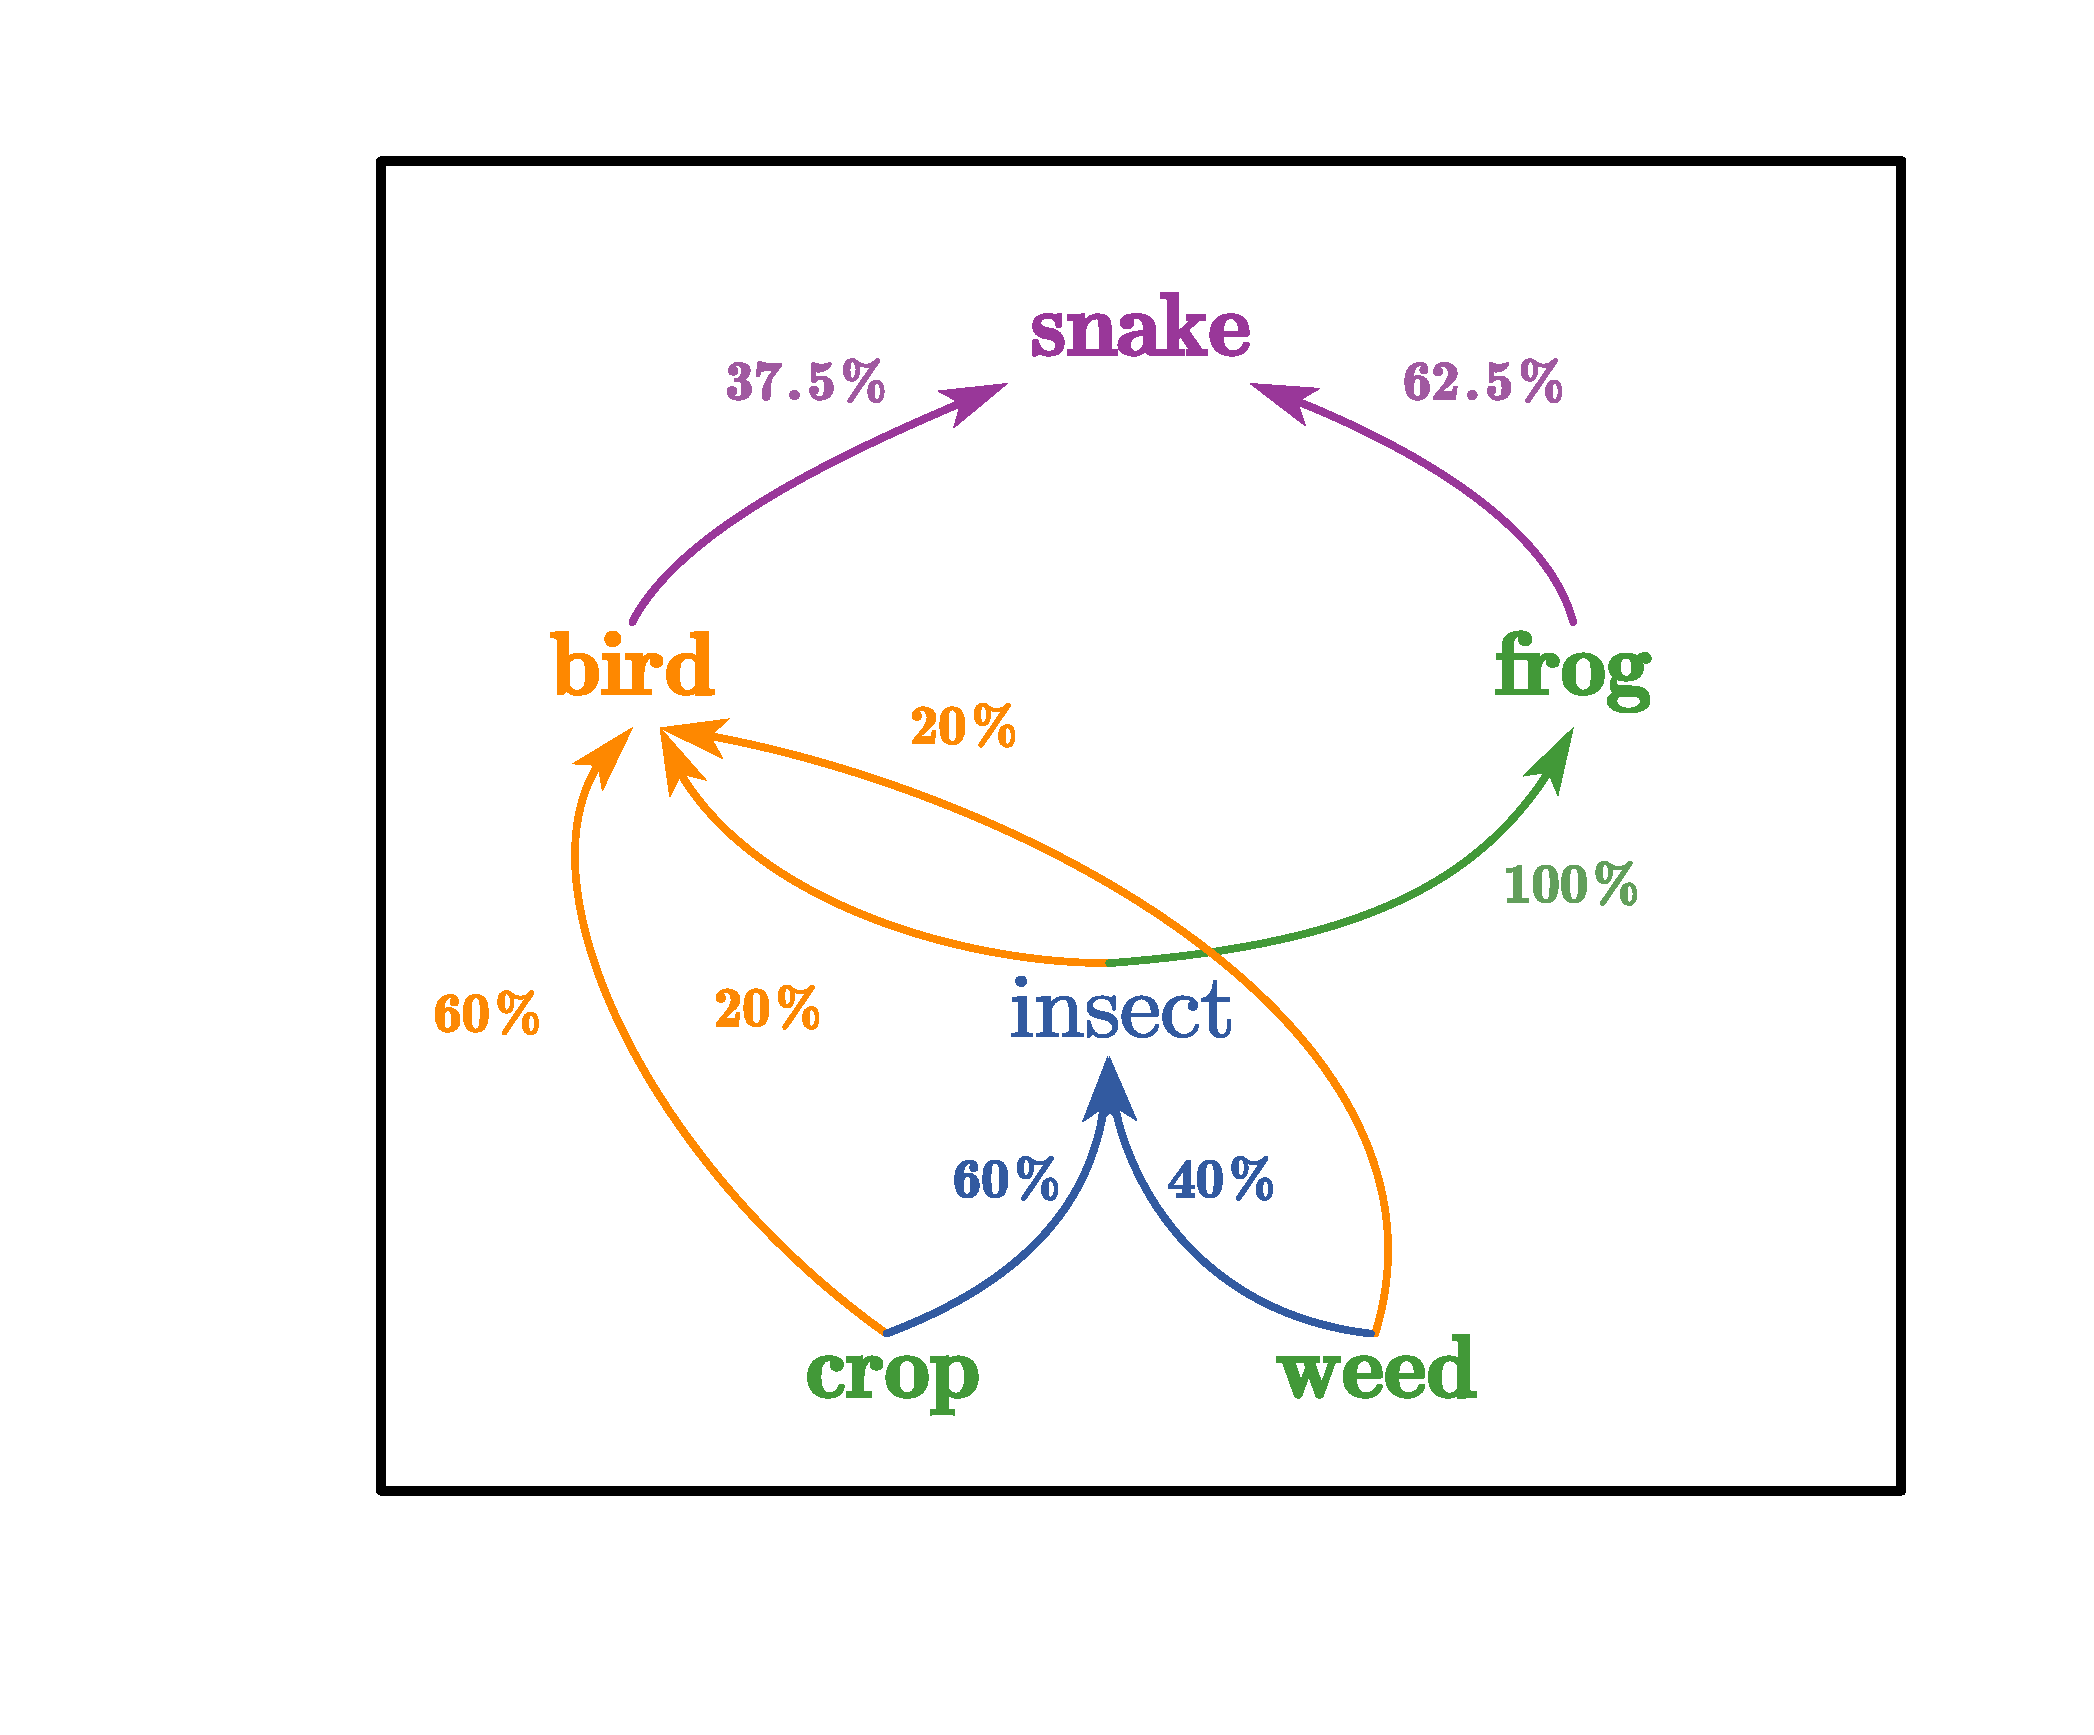
\includegraphics[height=6cm, keepaspectratio]{images/food_web_chem.pdf}
            \caption{Traditional Mode}
            \label{fig:food_web_chem}
          \end{minipage}
          \hspace{0.05\linewidth}
          \begin{minipage}[b]{0.45\linewidth}
              \centering
              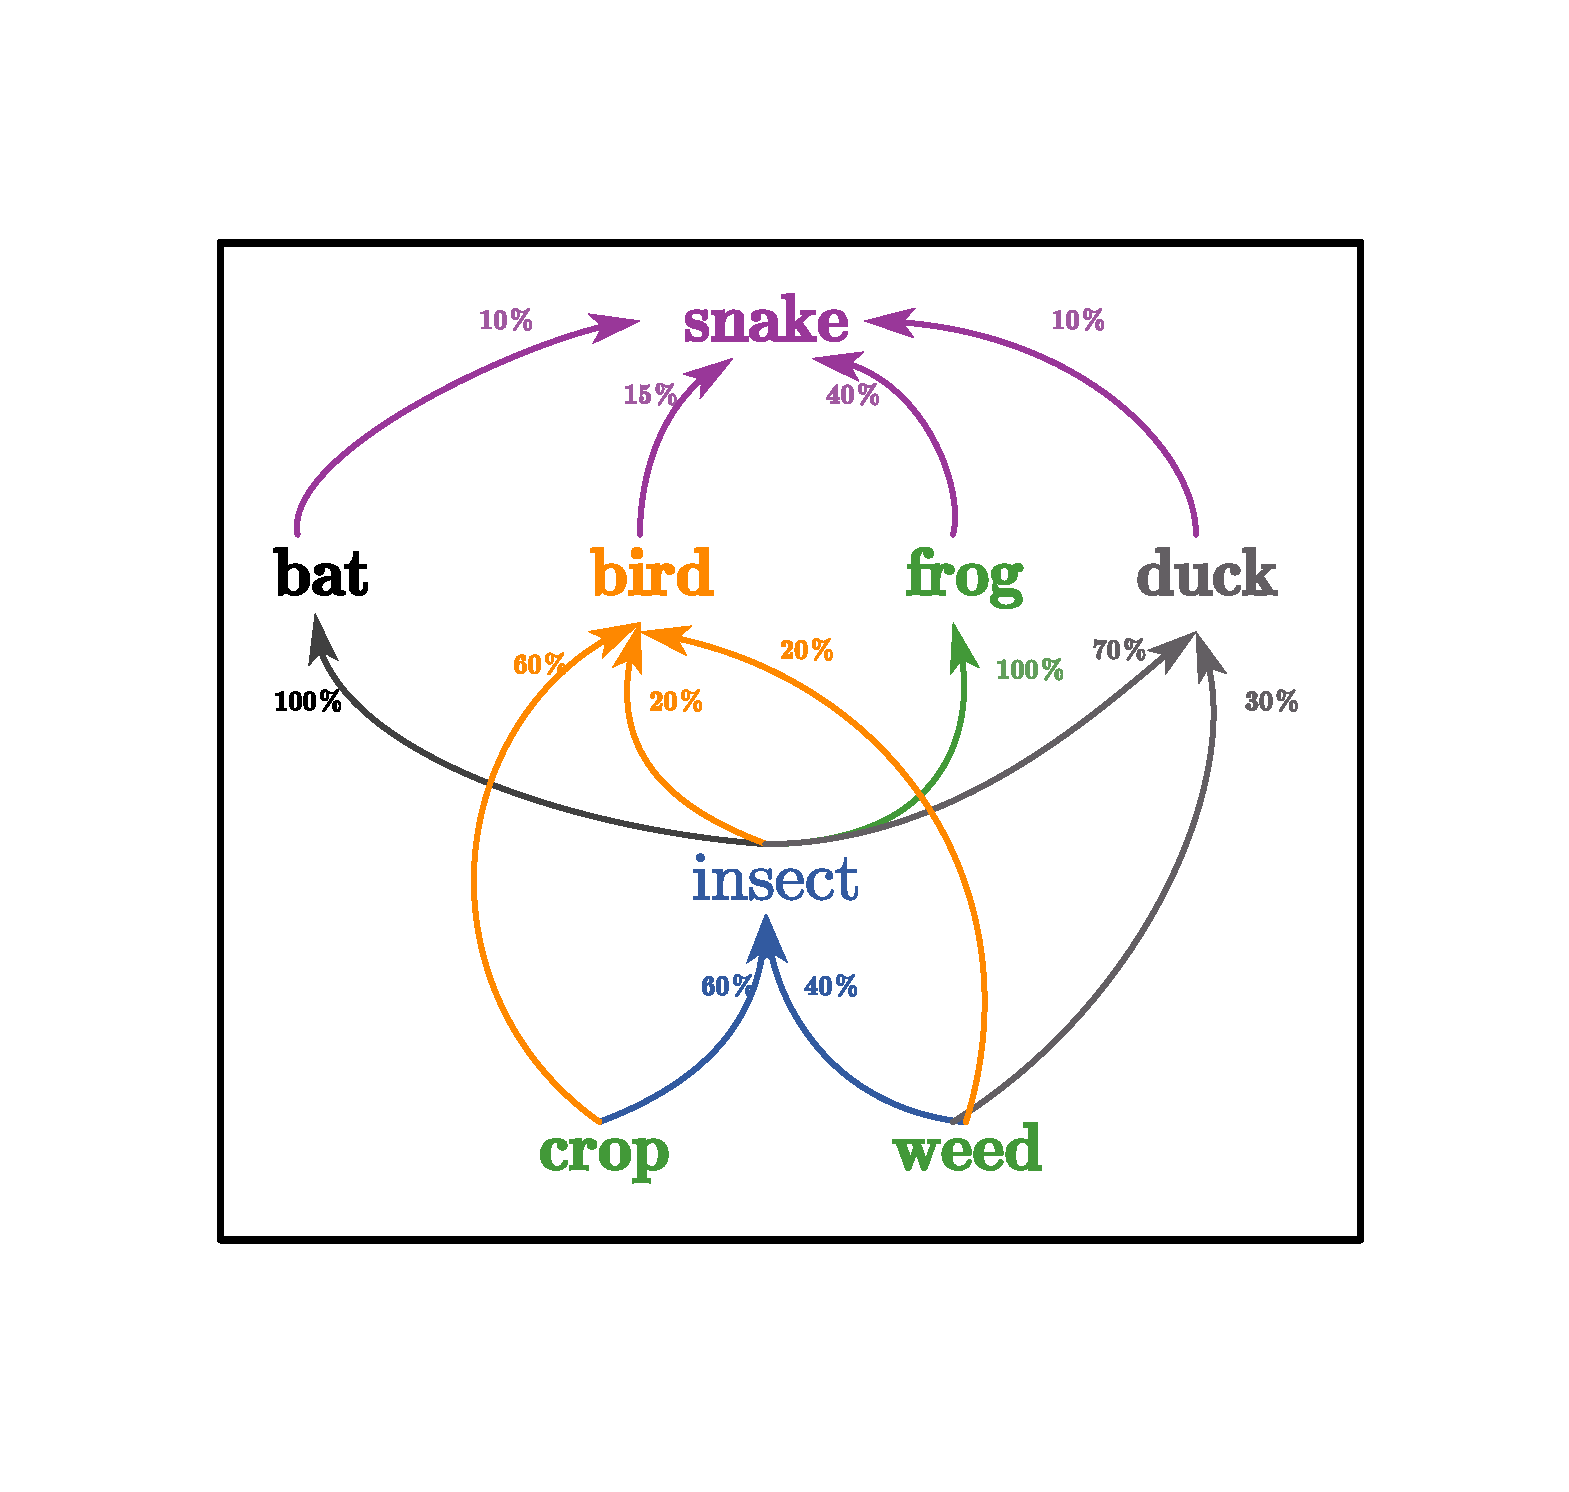
\includegraphics[height=6cm, keepaspectratio]{images/food_web.pdf} % 替换为你的第二张图片路径
              \caption{Green Mode}
              \label{fig:food_web_green}
          \end{minipage}
        \end{figure}
        
          We focus on comparing the dynamic behavior of the ecosystem in scenarios 
          where chemicals are used (conventional scenario) versus when a green agricultural plan is adopted (target scenario).

          The system comparison between using chemicals for pest control and using green agricultural methods is shown in Figure \ref{fig:S3S5}.

          \begin{figure}
            \centering
            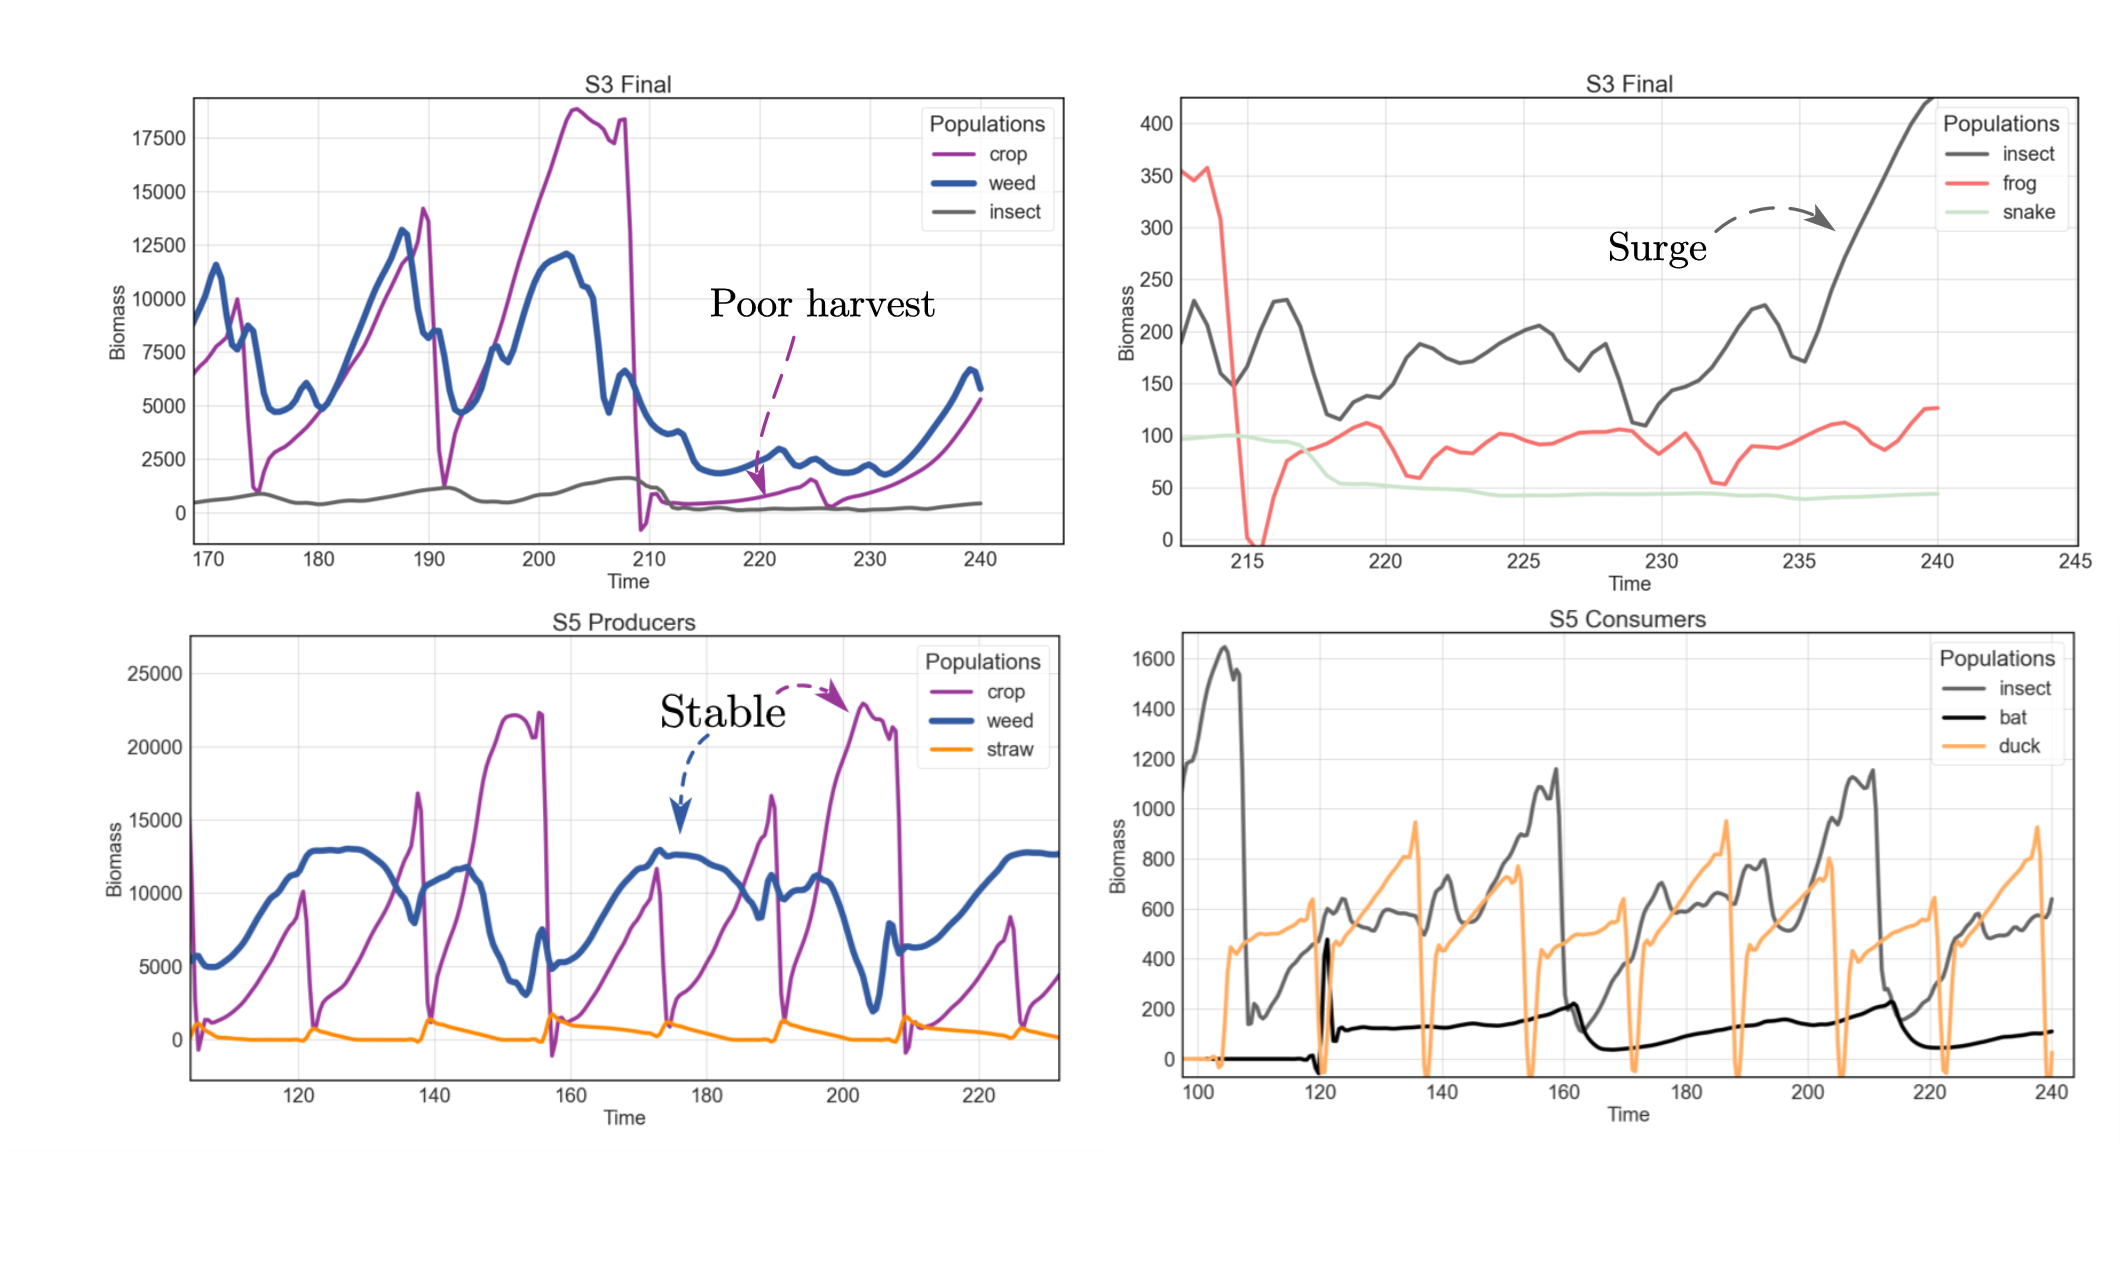
\includegraphics[width=\linewidth]{images/S3S5.png}
            \caption{Comparison between S3 and S5}
            \label{fig:S3S5}
          \end{figure}
          
          As discussed in the previous section, 
          when the green agricultural plan is not used, once chemicals are removed, 
          weeds and pests rapidly proliferate and compete with rice, eventually leading to the demise of the rice crop. 
          BeSides, the figure illustrates that there is a poor harvest between week 210 to week 240, even though chemicals are used, 
          which further prove the instability of chemical methods.
          However, if the green agricultural plan is adopted, even without chemicals, weeds and pests are effectively controlled, 
          and the system biomass fluctuates very little, maintaining a high level of stability. 
          This can also be explained by the niche theory previously discussed.
          
          In summary, when the model is applied to real-world scenarios, it aligns closely with actual ecological patterns, 
          demonstrating the model's versatility and accuracy.
      \subsection{Benifits Analysis}
        At the time of harvest, we assume that 30\% of the rice biomass is harvested as grain, 
        with a net profit of 0.5 USD per kilogram of grain. Additionally, we consider the harvest of ducks, 
        with a net profit of 1 USD per kilogram of duck, taking into account costs such as feeding. 
        
        Based on this, we can calculate the total value of the grain in each quarter under different scenarios, 
        as shown in Figure \ref{fig:Benefits}.
        \begin{figure}
          \centering
          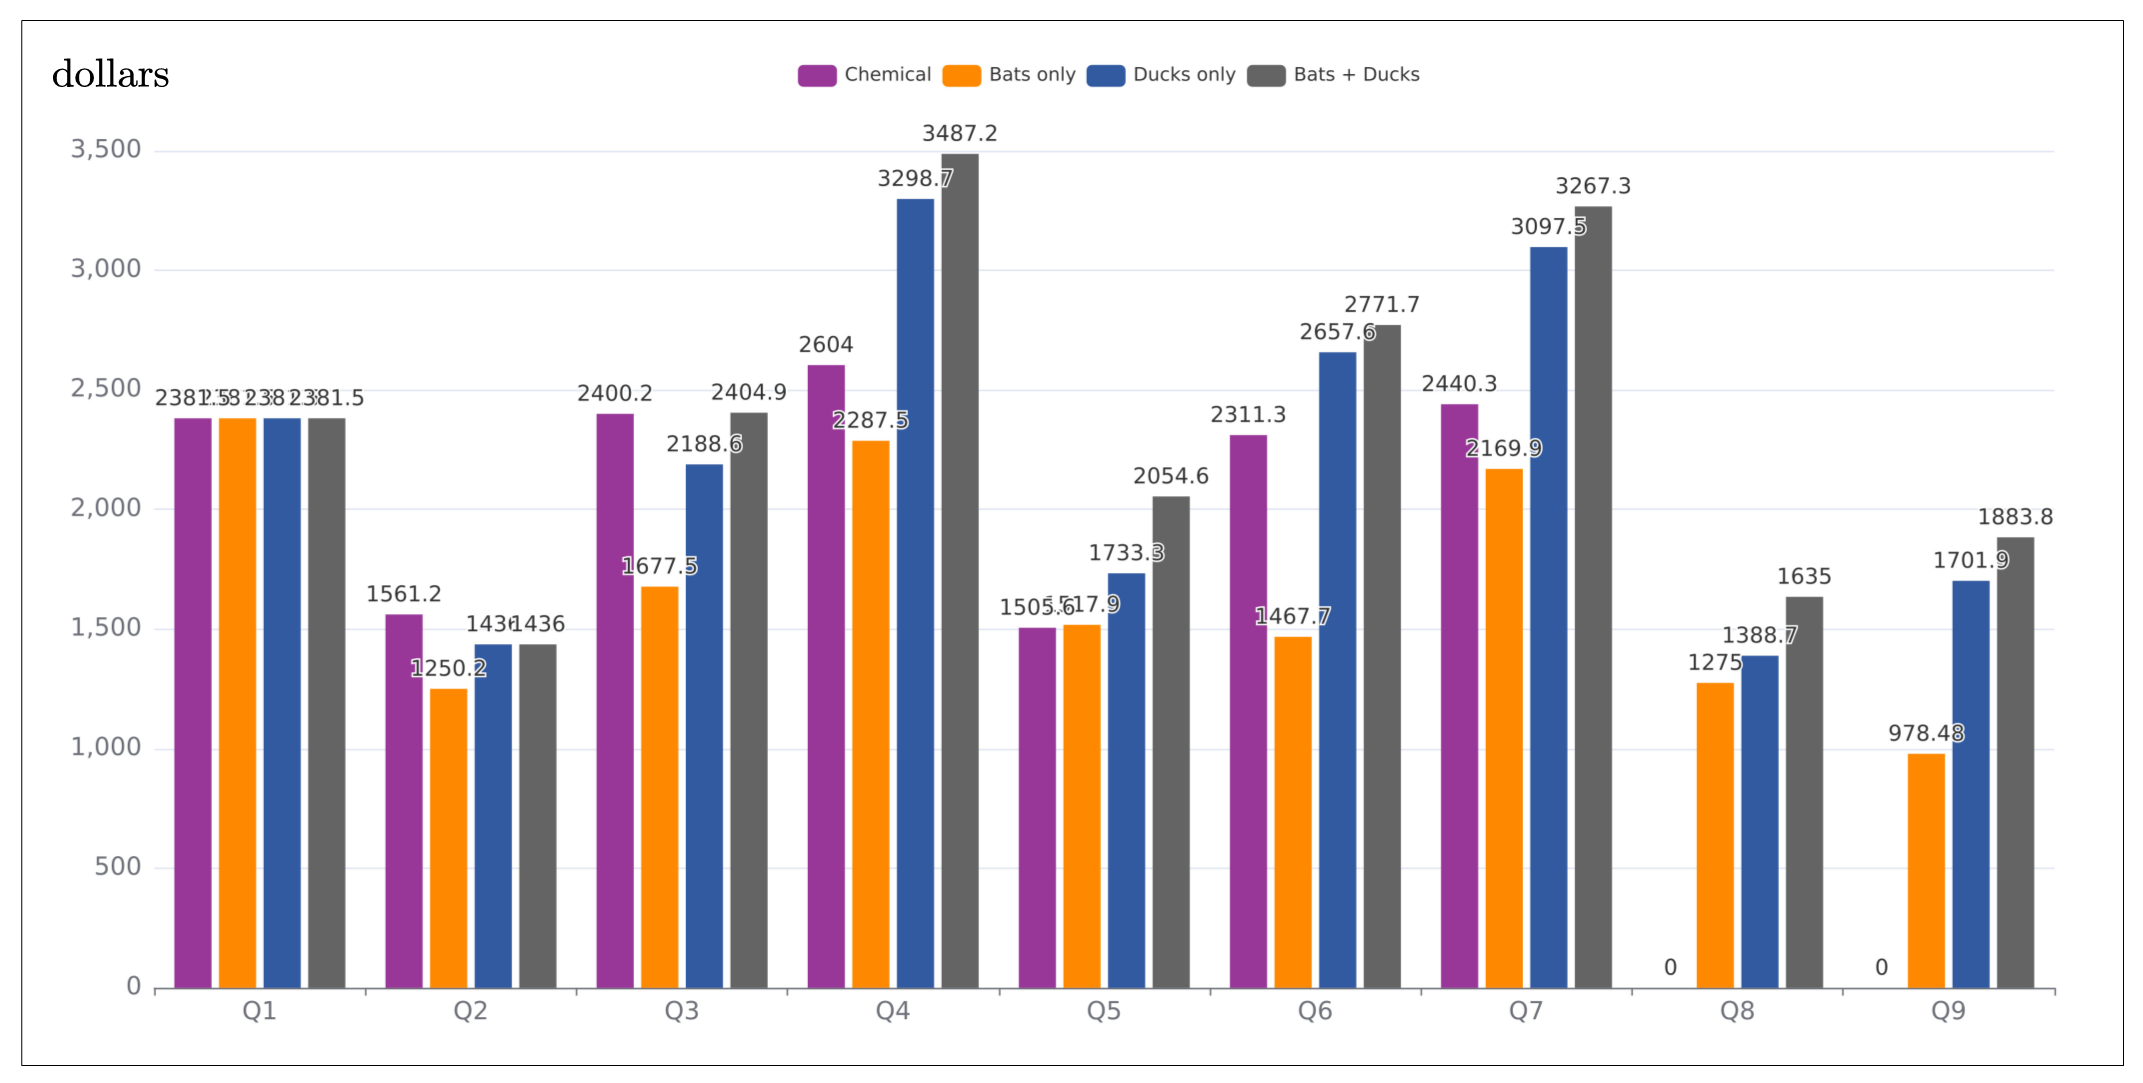
\includegraphics[width=\linewidth]{images/benefits_processed.png}
          \caption{Benenits of Each Senario}
          \label{fig:Benefits}
        \end{figure}
        Overall, bats play a crucial role in maintaining ecosystem stability, 
        as they both prey on insects and facilitate plant pollination. 
        While chemical agriculture may provide good returns in the short term, 
        its resilience to disturbances is relatively weak, 
        and external disruptions may eventually reduce profits to zero. 

        It is worth noting that the profit in the second cycle of every three cycles is the lowest. This is because the second cycle corresponds to the dry season, which highlights the strength of the seasonality component in our model. The seasonal variations in environmental conditions, such as water availability, significantly influence the ecosystem's productivity and, consequently, the profitability in different cycles. This feature of the model reflects the realistic influence of seasonal changes on agricultural systems, adding another layer of accuracy to our predictions.

        The introduction of ducks not only replaces the role of chemicals but also generates additional profits. 
        If considered in isolation, the profit from duck harvests is the highest. 
        However, when taking into account the comprehensive factors, 
        the combined introduction of both bats and ducks results in the maximum overall profit.
        

  \section{Sensitivity Analysis}
    We consider the effects of changes in two types of model parameters on the system: 
    the initial values of biomass density \( W \) in the dynamic model and typical environmental parameters. 
    The sensitivity analysis of the system is conducted over a time range of 0 to 80 weeks. 
    During this period, the agricultural ecosystem model corresponds to a chemical-use system that considers species re-migration (Model III). 
    Given that rice is the primary producer and crop in this agricultural ecosystem, 
    the figures in the following discussion use the time evolution of rice biomass as a representative example.

    \subsection{Changes in Initial Biomass Density}
      The initial values of all biomass densities \( W \) in the system are set to three different values: 
      the original values as shown in Chapter 4 figures, five times the original values, and 20\% of the original values. 
      These scenarios simulate the diversity of converted forest conditions and agricultural environments. 
      The resulting curves are shown in Figure \ref{fig:Change_init}.

      \begin{figure}[H]
        \centering
        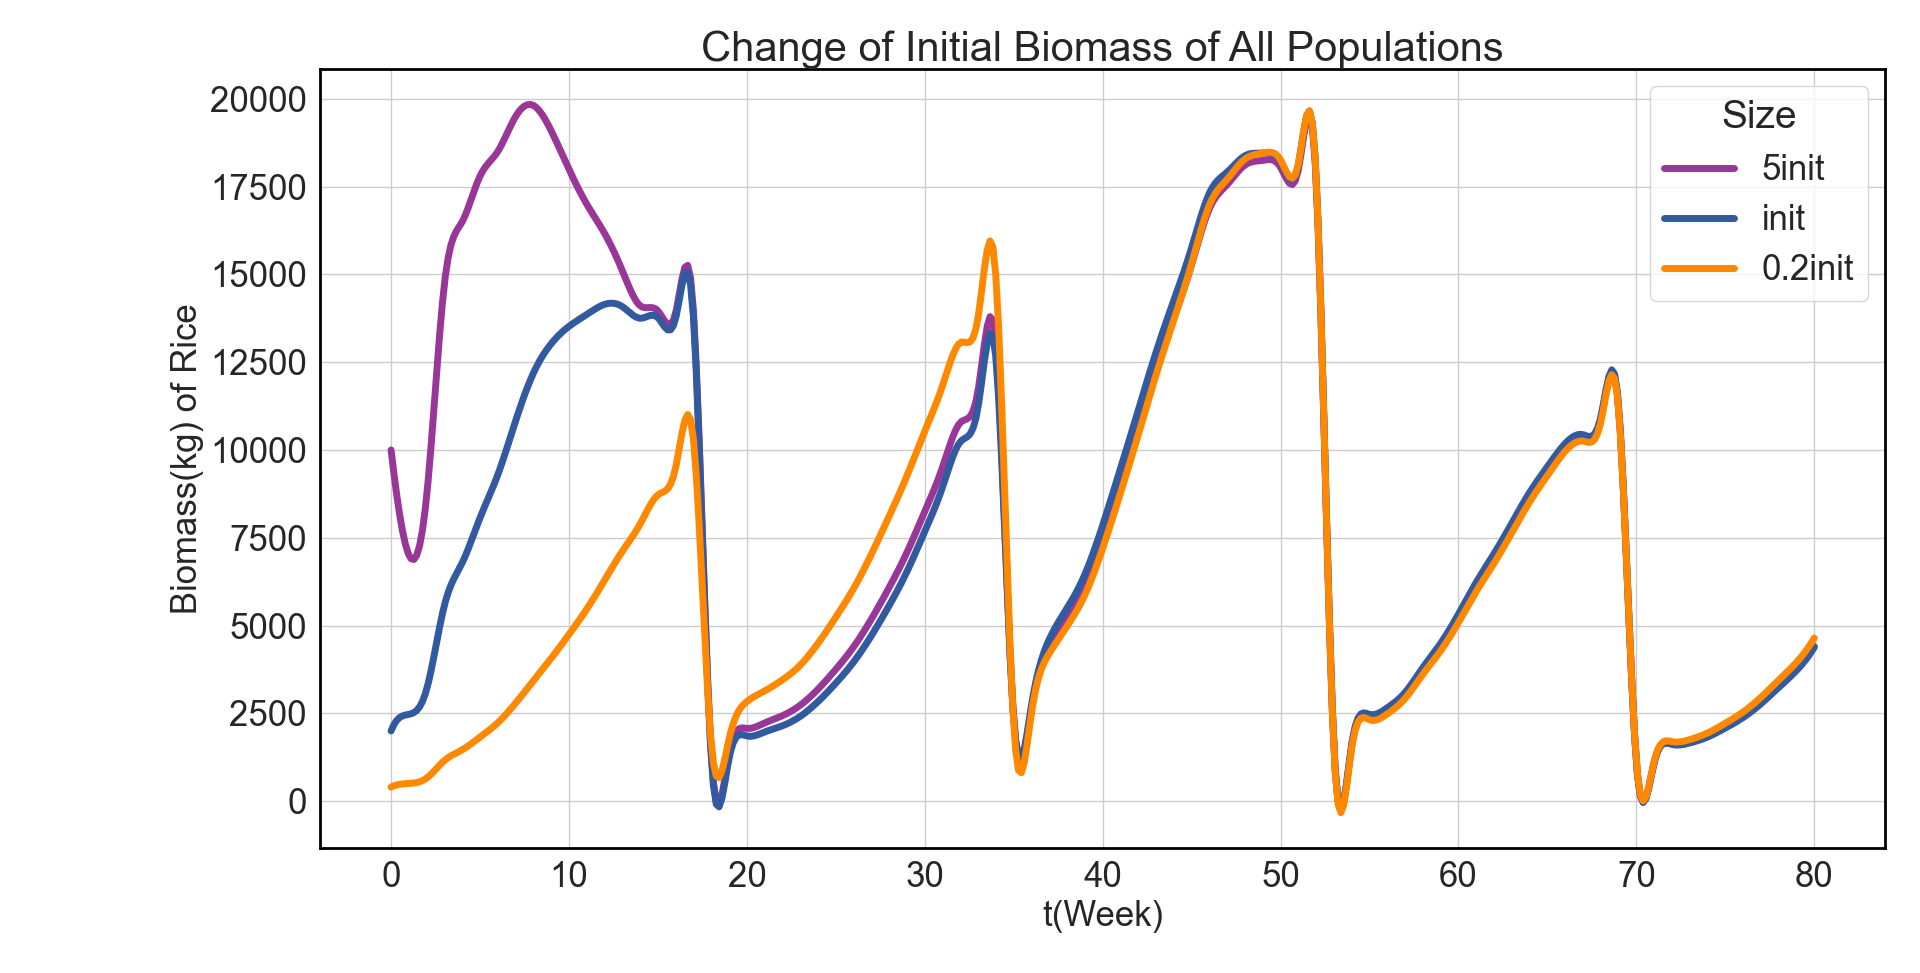
\includegraphics[width=0.75\linewidth]{images/Change_init.png}
        \caption{Impact of Initial Biomass Density Changes on System Dynamics}
        \label{fig:Change_init}
      \end{figure}

      From the figure, we observe that the biomass curves representing the three initial conditions converge after a relatively long period of natural evolution. 
      Similar patterns are observed for other populations in the ecosystem. 
      This demonstrates that our agricultural ecosystem model possesses a degree of self-regulation, 
      consistent with the stability and self-recovery capabilities of real-world ecological systems.

    \subsection{Changes in Typical Environmental Parameters}
      Let's examine the effects of changes in four typical environmental parameters that significantly influence the system: 
      the natural growth rate of rice biomass \( r_{crp} \), 
      the weed-to-rice competition coefficient \( \beta_{c\rightarrow w} \), 
      the environmental maximum biomass carrying capacity for rice \( \mathscr{K}_{crp} \), 
      and the standard deviation of Gaussian white noise \( \sigma \). 
      Each parameter is set to three different values (as indicated in the figures below), 
      and the resulting curves are plotted in Figure \ref{fig:Change_all}. 
      In the plots related to \( \beta_{c\rightarrow w} \), 
      we also include the time evolution of weed biomass for comparison with rice.

    \begin{figure}[H]
      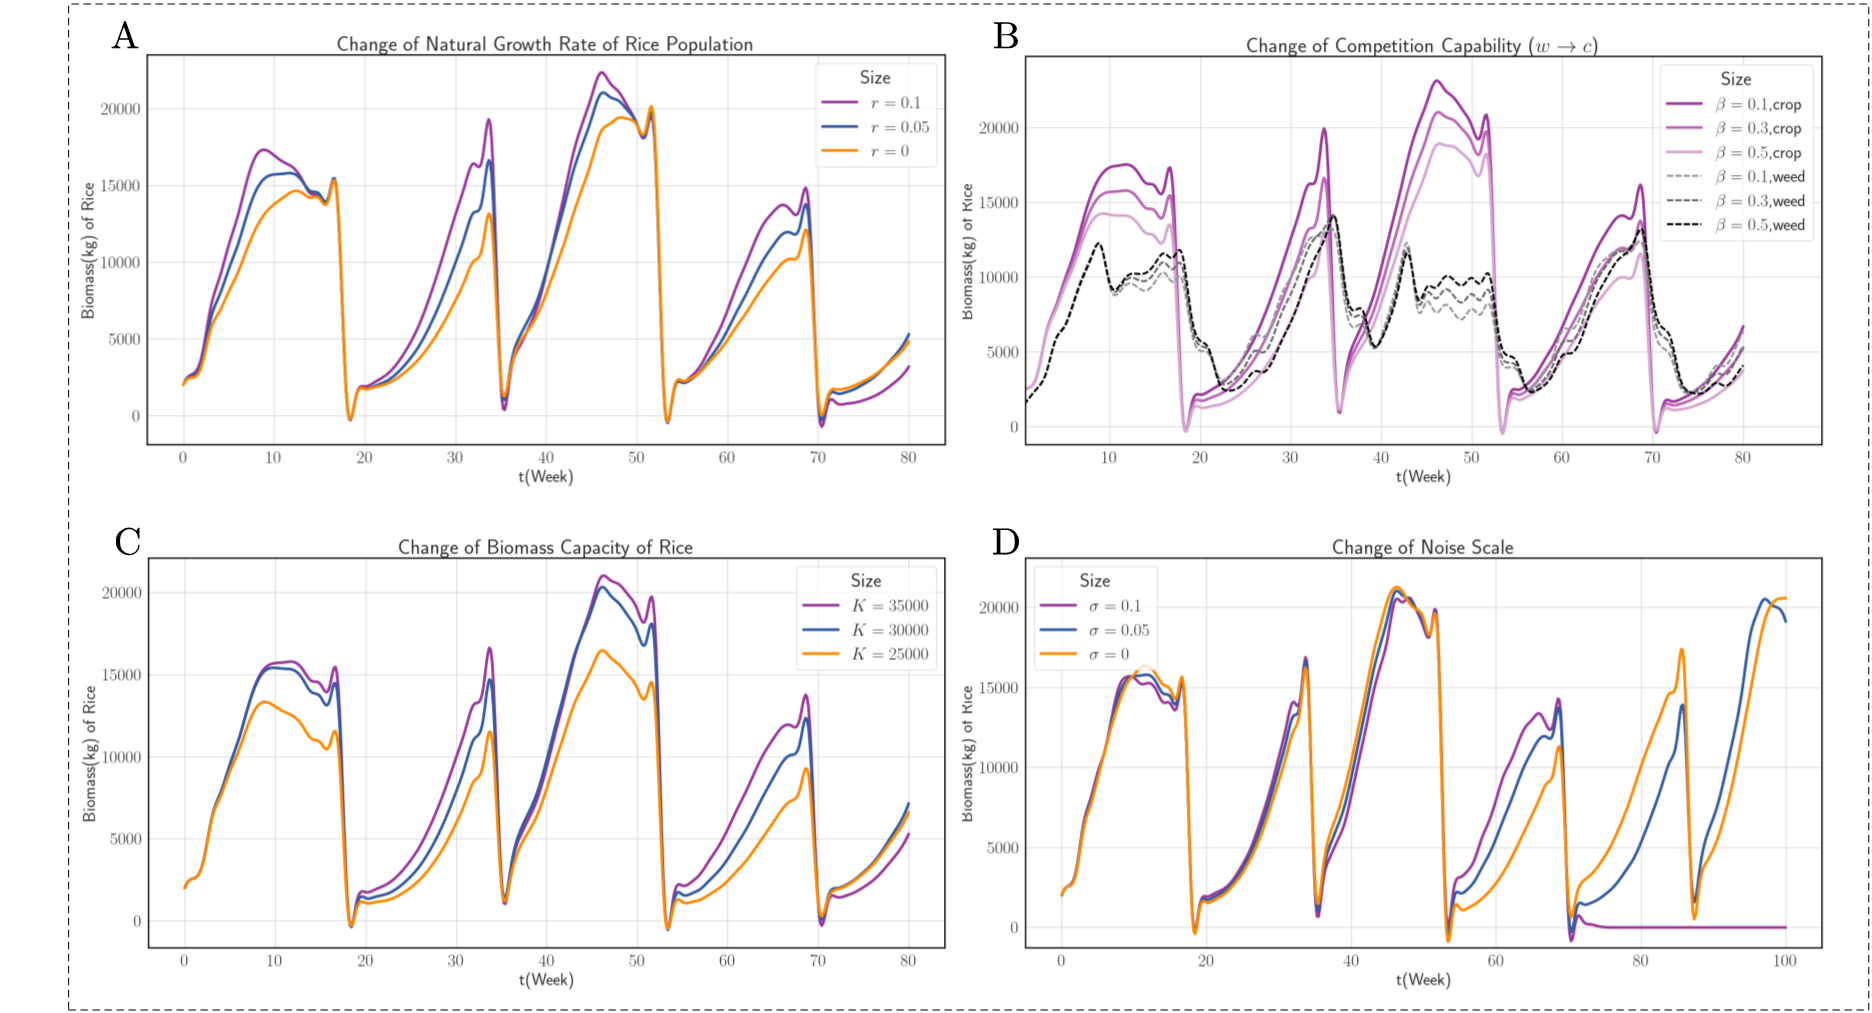
\includegraphics[width=\linewidth]{images/Change_all.png}
      \caption{Impact of Changes in Key Environmental Parameters on System Dynamics}
      \label{fig:Change_all}
    \end{figure}

    Below, we analyze the curves for each of the four scenarios:
    \begin{itemize}
      \item Effect of \( r_{crp} \) (natural growth rate of rice biomass):** 
      As shown in Figure \ref{fig:Change_all} (A), an increase in \( r_{crp} \) leads to an upward trend in rice biomass at any given time, and vice versa. 
      From an ecological perspective, an increase in \( r_{crp} \) indicates a higher marginal growth rate of rice biomass, resulting in faster growth, 
      which aligns with the figure. On the other hand, 
      the overall evolutionary trend of the system remains approximately the same when \( r_{crp} \) varies within a certain range, 
      reflecting the system's stability.
      \item Effect of \( \beta_{c\rightarrow w} \) (weed-to-rice competition coefficient):** As shown in Figure \ref{fig:Change_all} (B), 
      an increase in \( \beta_{c\rightarrow w} \) results in a downward trend in rice biomass and an upward trend in weed biomass at any given time, 
      and vice versa. Ecologically, an increase in \( \beta_{c\rightarrow w} \) reflects a higher competitive ability of weeds relative to rice, 
      enabling weeds to gain an advantage in interspecies competition, which is consistent with the figure. 
      Moreover, the overall evolutionary trend of the system remains approximately the same when \( \beta_{c\rightarrow w} \) varies within a certain range, 
      demonstrating system stability.
      \item Effect of \( \mathscr{K}_{crp} \) (maximum carrying capacity for rice):** As shown in Figure \ref{fig:Change_all} (C), 
      an increase in \( \mathscr{K}_{crp} \) results in an upward trend in rice biomass at any given time, and vice versa. 
      Ecologically, an increase in \( \mathscr{K}_{crp} \) indicates a higher potential maximum biomass for rice, 
      with rice biomass gradually approaching this value under suitable growth conditions, consistent with the figure. 
      Similarly, the overall evolutionary trend remains stable within a certain range of \( \mathscr{K}_{crp} \), further reflecting system stability.
      \item Effect of \( \sigma \) (standard deviation of Gaussian white noise):** As shown in Figure \ref{fig:Change_all} (D), 
      when \( \sigma \) is within a certain range, the trend of rice biomass over time remains approximately the same, 
      further demonstrating that the system's overall evolutionary trend is essentially unaffected. 
      Since \( \sigma \) is positively correlated with the amplitude of random fluctuations in the system, 
      this reflects the system's stability. However, it is noted that when \( \sigma = 0.1 \), rice goes extinct around week 70. 
      This occurs because large random fluctuations cause severe negative disturbances in the dynamics of rice biomass, 
      leading to its rapid decline to zero when the growth rate of \( W_{crp} \) is relatively low. 
      This illustrates that the system's stability and resilience to disturbances are finite, 
      which is consistent with the ecological concept of limited resistance and recovery in ecosystems.
    \end{itemize}
  \section{Evaluation of the Model}
    \subsection{Strengths}
    \subsection{Weaknesses}
  \section{Suggestions}

  %%citation
  % as \figurename~\ref{fig:image1} shows,this is a picture.
  % ...\cite{example1}
  % 123123123\cite{rosenow1983drought}

  \addcontentsline{toc}{section}{References}
  \bibliographystyle{unsrt}%{brief}%{alpha}%{unsrt}
  \bibliography{article_file}

\end{document}